\documentclass[preprint]{sig-alternate-05-2015}
\pagenumbering{arabic} % Remove for camera-ready

\usepackage{amsmath}
\usepackage{color}
\usepackage{xcolor}
\usepackage{colortbl}
\usepackage{listings}
\usepackage{multirow}
\usepackage{mdframed}
\usepackage{url}
\usepackage[subsubsection]{algorithm}
\usepackage{algpseudocode}
\usepackage[numbers,sort&compress]{natbib}
\usepackage{flushend}

\newtheorem{definition}{Definition}
\newtheorem{defn}{Definition}
\newtheorem{property}{Property}
\newtheorem{theorem}{Theorem}

\definecolor{LightCyan}{rgb}{0.88,1,1}
\definecolor{BluishGray}{RGB}{226,227,231}
\definecolor{LightGray}{gray}{0.95}
\definecolor{Gray}{gray}{0.85}


%\usepackage{enumitem}

\newcommand{\ti}{\textit}
\newcommand{\tb}{\textbf}


%\let\oldbibliography\thebibliography
%\renewcommand{\thebibliography}[1]{\oldbibliography{#1}
%\setlength{\itemsep}{0pt}} %Reducing spacing in the bibliography.

\lstset{
language=Ada,                % choose the language of the code
basicstyle=\tiny,       % the size of the fonts that are used for the code
%numbers=left,                   % where to put the line-numbers
%numberstyle=\footnotesize,      % the size of the fonts that are used for the line-numbers
%stepnumber=1,                   % the step between two line-numbers. If it is 1 each line will be numbered
%numbersep=5pt,                  % how far the line-numbers are from the code
backgroundcolor=\color{white},  % choose the background color. You must add \usepackage{color}
showspaces=false,               % show spaces adding particular underscores
showstringspaces=false,         % underline spaces within strings
showtabs=false,                 % show tabs within strings adding particular underscores
%frame=single,           % adds a frame around the code
tabsize=2,          % sets default tabsize to 2 spaces
captionpos=b,           % sets the caption-position to bottom
breaklines=true,        % sets automatic line breaking
breakatwhitespace=false,    % sets if automatic breaks should only happen at whitespace
escapeinside={\%*}{*)},          % if you want to add a comment within your code
numbers=right,
numbersep=-10pt,
numberstyle=\tiny,
}

\algrenewcommand{\alglinenumber}[1]{\scriptsize#1:}

\begin{document}

% Copyright
\setcopyright{acmcopyright}
%\setcopyright{acmlicensed}
%\setcopyright{rightsretained}
%\setcopyright{usgov}
%\setcopyright{usgovmixed}
%\setcopyright{cagov}
%\setcopyright{cagovmixed}


% DOI
\doi{10.475/123_4}

% ISBN
\isbn{123-4567-24-567/08/06}

%Conference
%\conferenceinfo{ASE '16}{September 3--7, 2016, Singapore}

%\acmPrice{\$15.00}

%
% --- Author Metadata here ---

%\conferenceinfo{ASE}{'16 Singapore}
%\CopyrightYear{2007} % Allows default copyright year (20XX) to be over-ridden - IF NEED BE.
%\crdata{0-12345-67-8/90/01}  % Allows default copyright data (0-89791-88-6/97/05) to be over-ridden - IF NEED BE.
% --- End of Author Metadata ---

\title{Fostering Software Architect\\and Programmer Collaboration}
%
% You need the command \numberofauthors to handle the 'placement
% and alignment' of the authors beneath the title.
%
% For aesthetic reasons, we recommend 'three authors at a time'
% i.e. three 'name/affiliation blocks' be placed beneath the title.
%
% NOTE: You are NOT restricted in how many 'rows' of
% "name/affiliations" may appear. We just ask that you restrict
% the number of 'columns' to three.
%
% Because of the available 'opening page real-estate'
% we ask you to refrain from putting more than six authors
% (two rows with three columns) beneath the article title.
% More than six makes the first-page appear very cluttered indeed.
%
% Use the \alignauthor commands to handle the names
% and affiliations for an 'aesthetic maximum' of six authors.
% Add names, affiliations, addresses for
% the seventh etc. author(s) as the argument for the
% \additionalauthors command.
% These 'additional authors' will be output/set for you
% without further effort on your part as the last section in
% the body of your article BEFORE References or any Appendices.

\numberofauthors{1} %  in this sample file, there are a *total*
% of EIGHT authors. SIX appear on the 'first-page' (for formatting
% reasons) and the remaining two appear in the \additionalauthors section.
%
\author{
\alignauthor
%Van Cam Pham, Shuai Li, Ansgar Radermacher, S\'ebastien G\'erard\\
%       \affaddr{CEA}\\
%       \affaddr{Address}\\
%       \affaddr{Saclay, France}\\
%       \email{first-name.last-name@cea.fr}
Anonymous Authors\\
       \affaddr{Institution}\\
       \affaddr{Address}\\
       \affaddr{City, State, Country}\\
       \email{Email}
}
\maketitle

\begin{abstract}
The so-called model-driven engineering approach relies on two paradigms, abstraction and automation, recognized as very efficient for dealing with complexity of today system. 
%Abstraction is the ability to provide simplified and focused view of a system and requires adequate modeling language. 
%For this concern, it is clear that the Unified Modeling Language (UML) is nowadays the most used, educated, documented and tooled modeling language. 
%Even, if a graphical language such as the UML is not the silver bullet for all software related concerns, it provides hence better support than text-based solutions for some concerns such as architecture and logical behavior of application development. 
UML state machine and their visual representations are much more suitable to describe logical behaviors of system entities than any equivalent text based description such as IF-THEN-ELSE or SWITH-CASE constructions. Although many industrial tools and research prototypes can generate executable code from such graphical language, their support only focus special cases of UML state machine, especially non-concurrent state machines. While UML state machine concepts such as concurrency, pseudo states such as history, fork, junction and time events are widely used by software architects, the code generation of the existing approaches does not take these concepts into account. To blur the boundaries between the modeling and coding worlds, a code generator should be able to generate code from all concepts of modeling languages with respect to the semantics described by the language specifications.

To this end, this paper proposes an approach to generate code from all UML state machines with all of its concepts with respect to the Precise Semantics of UML, especially concurrent state machines which are based on multi-thread-based design.
%After code modifications, round-trip engineering is needed to make the model and code consistent, which is a critical aspect to meet quality and performance constraint required from project manager today. Unfortunately, current UML tools only support structural concepts for round-trip engineering such as those available from class diagrams. In this paper, we address the round-trip engineering of UML state-machine and its related generated code. We propose a round-trip engineering approach consisting of a forward process which generates code by using transformation patterns, and a backward process which is based on code pattern detection to update the original state machine model from the modified generated code. We implemented a prototype and conducted several experiments on different aspects of the round-trip engineering to verify the proposed approach.
%\lipsum[1]
\end{abstract}


%
% The code below should be generated by the tool at
% http://dl.acm.org/ccs.cfm
% Please copy and paste the code instead of the example below. 
%
\begin{CCSXML}
<ccs2012>
<concept>
<concept_id>10011007.10011074.10011081.10011082</concept_id>
<concept_desc>Software and its engineering~Software development methods</concept_desc>
<concept_significance>300</concept_significance>
</concept>
<concept>
<concept_id>10011007.10011074.10011134</concept_id>
<concept_desc>Software and its engineering~Collaboration in software development</concept_desc>
<concept_significance>300</concept_significance>
</concept>
%<concept>
%<concept_id>10011007.10011074.10011111.10003465</concept_id>
%<concept_desc>Software and its engineering~Software reverse engineering</concept_desc>
%<concept_significance>100</concept_significance>
%</concept>
</ccs2012>
\end{CCSXML}

\ccsdesc[300]{Software and its engineering~Software development methods}
\ccsdesc[300]{Software and its engineering~Collaboration in software development}
%\ccsdesc[100]{Software and its engineering~Software reverse engineering}
%
% End generated code
%

%
%  Use this command to print the description
%
\printccsdesc

% We no longer use \terms command
%\terms{Theory}

\keywords{Round-trip engineering, Model-driven engineering, Model code co-evolution, UML, C++, Eclipse Modeling Tools}





\section{\uppercase{Introduction}}
\label{sec:intro}
%1. Say the complexity, CPS .. UML SM is ...
%2. MDE ..., OMG defines powerful specification for USM..
%3. To blur the boundaries between... => need to have code generation
%4. Problem: 1. most of existing... focus only on sequency aspect..., many pseudo states are not supported while these pseudo states are widely used as powerful means to describe the dynamic behavior of system. 2. Concurrency is not taken into account. 3. Generated code is dependent on library of generation tools => not portable. Speed + executable size + runtime execution memory consumptio (for IoT)n + semantic conformance.
%To.... => this paper address the analysis for multithread-based concurrency code genration and the code generation for full UML state machine with respect to the specification...
%Contribution: Concurrency, systematic approach for code generation, evaluation conforming to UML precise semantics...
%Structure

%Internet of Things \cite{Li2015} drives the complexity of embedded systems today rapidly increases. 
%Today embedded systems directly interacting with running environment does not run in standalone mode but also react to the system environment changes. 
%Event-driven architecture \cite{Michelson2006} is an useful way to design such systems, in which events come to the system either from outside (data) or inside the system itself (time event or internal changes). 
The UML State Machine (USM) \cite{Specification2007} and its visualizations are efficient to model the behavior of event-driven architecture.   
%USM defines how systems behave in case of changes. 
%The rise in use of the Model-Driven Engineering (MDE) approach promotes the automation in software development. 
Tools and approaches are proposed to automatically translate USMs into executable code in the context of Model-Driven Engineering (MDE) \cite{Mussbacher2014}.%, which are recognized as very efficient for dealing with system complexity. 
%Automation is to reduce the gap between the modeling world
%, which consists of software architects, who prefer using graphical languages such as USM, 
%and the implementation world
%, which involves programmers 
%by bringing the ability to automatically generating code from diagram-based modeling languages such as USM to executable code.  
%The gap between the modeling world, which consists of software architects, who prefer using graphical languages such as USM, and the implementation world, which involves programmers, is therefore reduced. 

However, despite many advantages of MDE and USM, they are not widely adopted as a recent survey revealed \cite{1030}.
This is partially due to poor support for code generation \cite{forward2010perceptions}.

On one hand, the usefulness and semantics of USM are being empowered by OMG by providing more concepts and their precise semantics such as pseudo states and composite state machines. 
On the other hand, existing code generation tools and approaches have some issues regarding completeness, semantics and efficiency of generated code. 
Existing approaches either support a subset of USM modeling concepts or handle composite state machines by flattening into simple ones with a combinatorial explosion of states, and excessive generated code \cite{badreddin2014enhanced}.
%is language-dependent and still limited to simple cases, especially when considering concurrency of \ti{doActivity} and orthogonal regions, pseudo states such as history, and different events. 
%This again enlarges the gap between the USM semantics and the actual generated code.
Specifically, the following lists some of the current issues: 
\vskip 0.1cm
\noindent
\tb{Completeness:} Existing tools and approaches mainly focus on the sequential aspect while the concurrency of state machines is limitedly supported. 
Pseudo states are not rigorously supported by existing tools such as Rhapsody 
	%does not support \ti{doActivity}, junctions, and truly concurrent execution of orthogonal regions
	\cite{ibmdiff}.
	%Concurrency of is often implemented sequentially. 
	%Sinelabore \cite{sinelabore} does not support fork, join, junction and concurrent states. 
	%Rhapsody and Enterprise Architect \cite{EA} only support \ti{CallEvent} and \ti{TimeEvent} while \ti{SignalEvent} and \ti{ChangeEvent} are missing. 
	%Pseudo states such as history, choice and junction are poor \cite{EA,sinelabore} while these are very helpful in modeling.
Designers are then restricted to a subset of USM concepts during design.

\vskip 0.1cm
\noindent	
\tb{Efficiency:} Code generated from tools such as Rhapsody \cite{ibm_rhapsody} and FXU \cite{Pilitowski2007} depends on the libraries provided by the tool vendor, which makes the generated code non portable. 
Event processing speed and executable file size of generated code are not optimized \cite{6195875}.
	
\vskip 0.1cm
\noindent
\tb{Semantics:} The semantics of UML State Machine is defined by a recent OMG-standardized: Precise Semantics of State Machine (PSSM) \cite{OMG2015}.
This standard is not (yet) taken into account for validating the runtime execution semantics of generated code. 

%In order for wider integrating MDE into software development today, one task is to seamlessly make the behavior of the code generated from UML State Machine complied with the semantics specified by PSSM. 
Given the above issues, the objective of this paper is to present a novel code generation pattern and its tooling support. 
The latter offers efficient code generated from USMs with full concepts to reduce the modeling-implementation gap.   

The proposed pattern extends IF-ELSE constructions with our support for concurrency. 
%The tool also supports \ti{deep separation} for separating USM-prescribed code and user action code,
Runtime execution of generated code is experimented with the PSSM test suite.
%Although supporting multi-thread-based concurrency, binary files compiled from and the event processing speed of runtime execution of code generated by our approach are dramatically smaller than some manual implementation approaches and code generation tools.
  
%Abstraction provides simplified and focused views of a system and requires adequate graphical modeling languages such as Uni. Even, if the latter is not the silver bullet for all software related concerns, it provides better support than text-based solutions for some concerns such as architecture and logical behavior of application development. UML state machines (USMs) and their visual representations are much more suitable to describe logical behaviors of system entities than any equivalent text based descriptions. The gap from USMs to system implementation is reduced by the ability of automatically generating code from USMs  \cite{Booch1998, Douglass1999,Shalyto2006,Douglass1999}. 

%Ideally, a full model-centric approach is preferred by MDE community due to its advantages \cite{Selic2012}. However, in industrial practice, there is significant reticence \cite{Hutchinson:2011:MEP:1985793.1985882} to adopt it.
%On one hand, programmers prefer to
%use the more familiar textual programming language. 
%On the other hand, software architects, working at higher levels
%of abstraction, tend to favor the use of models, and therefore
%prefer graphical languages for describing the architecture of
%the system.
%However, on the one hand, maintaining code generated from existing approaches is non-trivial. On the other hand our observation is that it is very difficult to come up with formalizations that yield such elegant code generation solutions \cite{6032552}. In other words, generated code must be manually modified to build fully operational applications. 
%On one hand there are traditional developers who prefer to implement the system by writing code, while on the other hand there are developers who prefer to use entirely models for the design and implementation of the system. 
%The code modified by programmers and the model are then inconsistent. Round-trip engineering (RTE) \cite{Hettel2008} is proposed to synchronize different software artifacts, model and code in this case \cite{Sendall}. RTE enables actors (software architect and programmers) to freely move between different representations \cite{Sendall} and stay efficient with their favorite working environment. 

%After code modifications, round-trip engineering (RTE) is needed to make the model and code consistent, which is a critical aspect to meet quality and performance constraint required from project managers today. 
%Unfortunately, current industrial tools such as for instance Enterprise Architect \cite{sparxsystems_enterprise_2014} and IBM Rhapsody\cite{ibm_rhapsody} only support structural concepts for RTE such as those available from class diagrams and code. Compared to RTE of class diagrams and code, RTE of USMs and code is non-trivial. It requires a semantical analysis of the source code, code pattern detection and mapping patterns into USM elements. 
%This is a hard task, since mainstream programming languages such as C++ and JAVA do not have a trivial mapping between USM elements and source code statements.

%For software development, one may wonder whether this RTE is doable. That is, why do the industrial tools not support the propagation of source code modifications back to original state machines? Several possible reasons to this lack are (1) the gap between USMs and code, (2) not every source code modification can be reverse engineered back to the original model, and (3) the penalty of using transformation patterns facilitating the reverse engineering that may not be the most efficient (e.g. a slightly larger memory overhead). 
%in the mind of these tools' vendors, users always make changes to models rather than to code. Generated code, in these tools, is therefore not supposed to be changed directly.  

%In this paper, we address the RTE of UML State Machine diagrams and its related generated code. We propose a RTE approach consisting of a forward process which generates code by using transformation patterns, and a backward process which is based on code pattern detection to update the original state machine model from the modified generated code. From the proposed approach, we implemented a prototype and conducted several experiments on different aspects of the round-trip engineering to verify the proposed approach. 



%Model-driven engineering (MDE) is a development methodology aiming to increase software productivity and quality by allowing different stakeholders to contribute to the system description \cite{Mussbacher2014}. MDE considers models as first-class artifacts and generates code from higher abstraction level models. Recent survey \cite{1030} has revealed that industries are gaining the adoption of code generation into software development life-cycle. Although many tools and research prototypes can generate executable code from models, generated code could be manually modified by programmers, e.g. skeleton code generated from UML \cite{Specification2007} class diagrams. Models and the generated code are therefore out of synchronization. Round-trip engineering \cite{Aßmann200333, Hettel2008, E-ESE-120044648} (RTE) is proposed to keep the artifacts synchronized.

%RTE supports synchronizing different software artifacts, model and code in this case, and thus enabling actors (software architect and programmers) to freely move between different representations \cite{Sendall}. Tools such as for instance Enterprise Architect \cite{sparxsystems_enterprise_2014}, Visual Paradigm \cite{visual}, and AndroMDA \cite{_andromda_} provide RTE but most of them are only applicable for system structure models such as class diagrams.  

%This study addresses the RTE of UML State Machine (SM) and object-oriented programming languages such as C++ and JAVA. SM is widely used in practice for modeling the behavior of complex systems, notably reactive, real-time embedded systems. There are several approaches to generating source code from state machines or state charts such as nested switch/if statements \cite{Booch1998}, state-event-table \cite{Douglass1999, Duby2001}, and state pattern \cite{Allegrini2002,Shalyto2006,Douglass1999}. Unfortunately, the generated code from these approaches is very difficult for programmers to maintain without an appropriate supporting tool. RTE is impossible in these approaches even with very small changes such as changing transition targets or actions made to code. The reason behind this impossibility is that, in mainstream programming languages such as C++, JAVA, (1) there are not equivalents between SMs and source code statements and (2) the code generation pattern of these approaches has not been chosen with RTE in mind.

%This paper addresses the RTE of UML state-machines and object-oriented programming languages such as C++ and JAVA. The forward  engineering of the approach takes as input a state-machine and executes two transformations. The first is UML to UML by utilizing several transformation patterns such as the double-dispatch approach presented in \cite{spinke_object-oriented_2013} and the second is a generation of code from the transformed UML. Traceability information is stored, during the transformations. In the backward direction, a verification is executed by the code pattern detection to verify the correctness of the code before the backward process taking as input the modified generated code, the UML classes, the original state-machine and mapping information together merges changes from code to the state-machine. We implemented a prototype supporting RTE of state-machine and C++ code, and conducted several experiments on different aspects of the RTE to verify the proposed approach. To the best of our knowledge, our implementation is the first tool supporting RTE of SM and code. 
%The prototype also improves the collaboration between MDE developers and traditional programmers in developing reactive complex embedded systems.

%This paper addresses the RTE of USMs and object-oriented programming languages such as C++ and JAVA. The main idea is to utilize transformation patterns from USMs to source code that aggregates code segments associated with a USM element into source code methods/classes rather than scatters these segments in different places. Therefore, the reverse direction of the RTE can easily statically analyze the generated code by using code pattern detection and maps the code segments back to USM elements. Specifically, in the forward direction, we extend the double dispatch pattern presented in \cite{spinke_object-oriented_2013}. Traceability information is stored during the transformations. We implemented a prototype supporting RTE of state-machine and C++ code, and conducted several experiments on different aspects of the RTE to verify the proposed approach. To1 the best of our knowledge, our implementation is the first tool supporting RTE of SM and code. 

To sum up, the contributions of this paper are: (1) an approach and tooling support for code generation from USMs with full features; 
(2) an empirical study on the semantic-conformance and efficiency of generated code;
and (3) application of the tool to a case study.  

We assume that readers of this paper have knowledge about UML State Machine and its basic execution semantics.

The remaining of this paper is organized as follows: Section \ref{sec:modeling} describes the modeling of applications using UML State Machines. 
Section \ref{sec:uniqueness} mentions the features of our tool.
Thread-based concurrency is designed in Section \ref{sec:thread}. 
Based on this design, a code generation approach is proposed in Section \ref{sec:codegen}. 
The implementation and empirical evaluation are reported in Section \ref{sec:exp}. 
The application of our tool to a case study is presented in Section \ref{sec:casestudy}.
Section \ref{sec:relatedwork} discusses related work. The conclusion and future work are presented in Section \ref{sec:conclusion}.

%\section{Motivating example}
\label{sec:example}
\begin{figure}
	\centering
	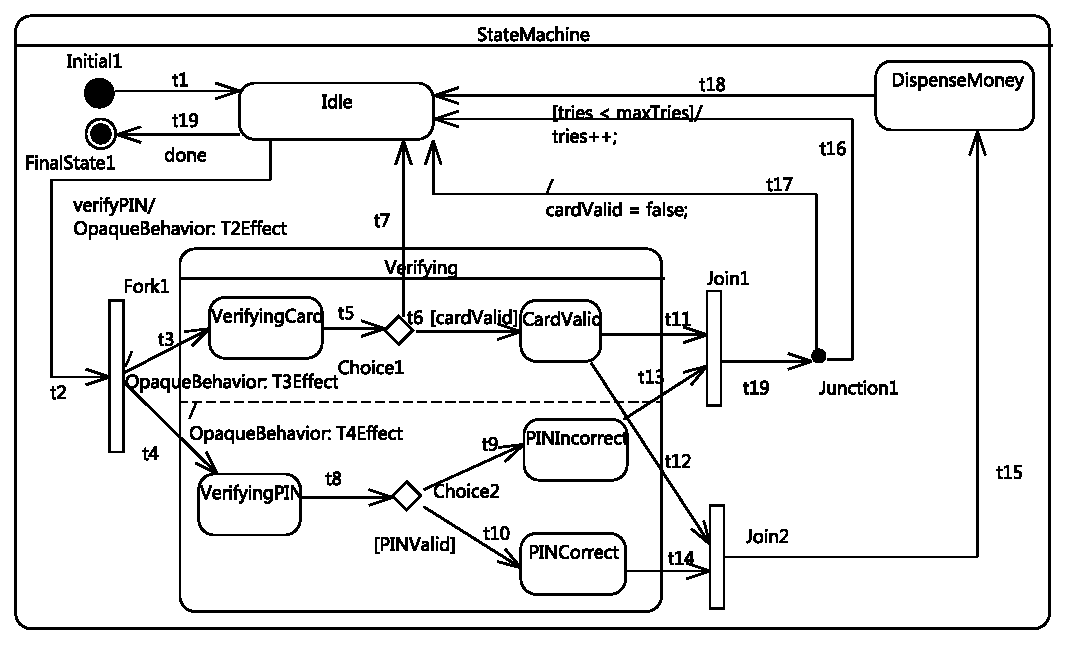
\includegraphics[clip, trim=0.2cm 0.2cm 0.2cm 0.2cm, width=1.0\columnwidth]{figures/ATM.pdf}
	\caption{ATM State machine example} 
	\label{fig:example}
\end{figure}

\section{Background definition}
\label{subsec:background}

%\begin{definition}A directed graph $G = \{V, Ed\}$ consists of a finite set $V$ of vertexes, and a set $Ed$ of edges. An edge connects a source vertex to a target vertex. The source and target vertexes of an edge ed are obtained by $src(ed)$ and $tgt(ed)$.
%\end{definition}

\begin{definition}A UML vertex $v \in V$ has a kind $v.kind \in$  \ti{\{initial, final, state, comp, conc, join, fork, choice, junction, enpoint, expoint, history\}}. 
\end{definition} 

\begin{definition}A region $r \in \mathcal{R}$ is composed of one or several vertexes, and contained by a state $s$. We write $owner(r) = s$ and $vertices(r)$ is its sub-vertices set. 
\end{definition}	

\begin{definition} A vertex is either a UML state or a pseudo-state. A UML state $s$ is a vertex and $s.kind$ $\in$ \{state, comp, conc\}. $s$ has an $entry$, an $exit$ and a $doActivity$ action. A composite state $cs$ contains one or more vertexes. We write $vertices(cs)$ is a set of vertexes contained by $cs$ and, inversely, $owner(v)$ refers to the containing state of the vertex $v$. %A concurrent state contains more than one region.
\end{definition}		

\begin{definition} An action $act$ $\in$ $ActLang$ is a set of statements written in an object-oriented programming language $ActLang$. A guard is a boolean expression written in $ActLang$.
\end{definition}

\begin{definition} A transition $t \in T$ is an edge connecting two vertexes. 
	The source and target vertexes of an edge ed are obtained by $src(t)$ and $tgt(t)$. 
	A transition has a guard $guard(t)$, an effect $effect(t)$, and is associated with a set of events $\subset$ E. We write $events(t)$ as the associated set of events. A transition has a type $t.type$ $\in \{trig, tless, gdless, triggdless\}$ and a kind $t.kind \in {external, local, internal}$.
\end{definition}

\begin{definition} An event is one of the followings:
	\begin{itemize}
		\item A \ti{TimeEvent} $te$ specifies the time of occurrence $d$ relative to a starting time. The latter is specified when a state, which accepts the time event, is entered.
		
		\item A \ti{SignalEvent} $se$ is associated with a signal $sig$, whose data are described by its attributes and is occurred if $sig$ is received by a component, which is an active UML class.
		
		\item A \ti{ChangeEvent} $che$ is associated with a boolean expression $ex(che)$ written in $ActLang$. $che$ is emitted if $ex(che)$ changes from true (false) to false (true).
		
		\item A \ti{CallEvent} $ce$ is associated with an operation $op(ce)$. $ce$ is emitted if there is a call to $op(ce)$.
	\end{itemize}
\end{definition}

\begin{comment}
\begin{definition} A \ti{TimeEvent} $te$ an internal event and specifies the time of occurrence $d$ relative to a starting time. The latter is specified when a state, which accepts the time event, is entered. 
\end{definition}

\begin{definition} A \ti{Signal} $sig$ is data described by its attributes. 
\end{definition}

\begin{definition} A \ti{SignalEvent} $se$ is associated with a signal $sig$ and is occurred if $sig$ is received by a component, which is an active UML class. 
\end{definition}	

\begin{definition}
	A \ti{ChangeEvent} $che$ is associated with a boolean expression $ex(che)$ written in $ActLang$. $che$ is emitted if $ex(che)$ changes from true (false) to false (true).
\end{definition}

\begin{definition}
	A \ti{CallEvent} $ce$ is associated with an operation $op(ce)$. $ce$ is emitted if there is a call to $op(ce)$.
\end{definition}
\end{comment}

Suppose that for each vertex \ti{v} $\in$ $V$, its incoming and outgoing transition lists are extracted by $T_{ins}(v)$ and $T_{outs}(v)$, respectively. %For a list $l$, the function $head$ is used to get the first element of the list. 
If $v.kind = conc$, suppose $regions(v)$ is the region set contained by $v$. %Given a transition t:
%\begin{itemize}
%	\item $t.type = trig$ if $\#events(t) > 0$.
%	\item $t.type = tless$ if $\#events(t) = 0$.
%	\item $t.type = gdless$ if $(guard(t) = true \vee \nexists guard(t)$.
%	\item $t.type = triggdless$ if $\#events(t) = 0 \wedge (guard(t) = true \vee \nexists guard(t))$.
%\end{itemize}

The behavior of an active class $C$ is described by using a state machine whose definition is as following:	

\begin{definition} A state machine sm is a graph specified by $\{V, T\}$ associated with a set of events $E$. A state machine is a special composite state which has no incoming and no outgoing transitions. A root vertex $v$ is a direct sub-vertex of the state machine, $owner(v) = sm$. The set of regions contained by $sm$ is written $\mathcal{R}$.
\end{definition}	

%For each vertex $v$ $\in$ $V$, we write the following sets $T_{ins} (v) = incomings(v), T_{outs}(v) = outgoings(v)$, $t_{first} = head(t_{outs})$; transitive transition sets $T_{ins}^{+}(v)$ and $T_{outs}^{+}(v)$ are sets of transitions incoming to and outgoing from, respectively, $v$ or direct or indirect sub-vertexes of $v$.

\begin{comment}
\begin{strip}
	\begin{equation}
	T_{ins}^{+} (v) =    \left\{
	\begin{array}{ll}
	T_{ins}(v) & v.kind \notin \{comp, conc\}  \\
	T_{ins}(v) \cup \bigcup\limits_{sub \in subvertexes(v)} T_{ins}^{+} (sub) & v.kind \in \{comp, conc\} \\
	\end{array} 
	\right.
	\end{equation}
	
	\begin{equation}
	T_{outs}^{+} (v) =    \left\{
	\begin{array}{ll}
	T_{outs}(v) & v.kind \notin \{comp, conc\}  \\
	T_{outs}(v) \cup \bigcup\limits_{sub \in subvertexes(v)} T_{outs}^{+} (sub) & v.kind \in \{comp, conc\} \\
	\end{array} 
	\right. 
	\end{equation}
\end{strip}
\end{comment}

\begin{definition} Transitive container $owner^+(v)$ of a vertex $v$ of a state machine $sm$ is defined as following:
	\begin{equation}
	owner^+(v) =    \left\{
	\begin{array}{ll}
	sm & owner(v) = sm \\
	owner(v) \cup owner^+(owner(v)) & otherwise\\
	\end{array} 
	\right.
	\end{equation}	
\end{definition}

Likewise, $vertices^+(v)$ is a set of transitive sub-vertexes.

\begin{comment}
In the example in Fig. \ref{fig:example}, we have:
\begin{IEEEeqnarray*}{lCr}	
	owner^+(Idle) = \{StateMachine\}, \\
	owner^+(Choice1) = \{Verifying, StateMachine\}.
\end{IEEEeqnarray*}
\end{comment}

%A state machine $sm = \{V, T\}$ is validated if an associated set of constraints is validated. 
%The set is not presented here due to space limitation.
%is validated if, for each $v \in V$, the constraints listed in Table \ref{table:constraint} are hold. %These are evaluated before the generation phase is taken into account. 

\begin{comment}
\begin{table*}
	\caption{State machine constraints}
	\label{table:constraint}
	\centering
	\begin{tabular}{|p{2.1\columnwidth}|}
	\hline	
	\tabitem If $v.kind = initial$ then $\#T_{outs}(v) = 1 \wedge \#T_{ins}(v) = 0 \wedge t_{first}.type = triggdless$. \\ 
	
	\tabitem If $v.kind = final$ then $\#T_{outs}(v) = 0$. \\
	
	\tabitem If $v.kind \notin \{state, comp, conc\}$ then $\forall t \in T_{outs}(v): src(t) \lnot= tgt(t)$. \\
	
	\tabitem If $T_{auto} = \{t \in T_{outs} | \#events(t) = 0\}$, $T_{ng} = \{t \in T_{auto} | guard(t) = true \vee \nexists guard(t)\}$ then $\#T_{ng} <= 1$. \\
	
	\tabitem $\#T_{ins}^+(v) > 0 \vee \#T_{outs}(v)^+ > 0$. \\
	
	\tabitem If $v.kind = comp$ then $\#subvertexes(v) > 0$. \\
	
	\tabitem If $v.kind = conc$ then $\#regions(v) > 0 \wedge (\forall r \in regions(v): \#subvertexes(r) > 0)$. \\
	
	\tabitem $\#regions(sm) = 1$. \\
	
	\tabitem If $v.kind = fork$ then $\#T_{ins}(v) > 0 \wedge \#T_{outs}(v) > 1 \wedge (\forall t \in T_{outs}(v): t.type = triggdless \wedge owner(tgt(t)).kind = conc)$. \\
	
	\tabitem If $v.kind = join$ then $\#T_{ins} > 1 \wedge \#T_{outs}(v) = 1 \wedge (\forall t \in T_{ins}(v): t.type = triggdless \wedge (\exists s \in owner^+(src(t)), s.kind=conc)) \wedge head(T_{outs}).type = triggdless$. \\
	
	\tabitem If $v.kind \in {choice, junction}$, then $\#T_{ins}(v) > 0 \wedge \#T_{outs}(v) > 1 \wedge (\exists! out \in T_{outs}(v): out.type = gdless)$. \\
	
	\tabitem If $v.kind \in {enpoint, expoint}$, then $owner(v).kind \in \{comp, conc\} \wedge \#T_{ins}(v) > 0 \wedge \#T_{outs}(v) = 1 \wedge head(T_{outs}(v).type = triggdless)$. \\
	
	\tabitem If $v.kind = history$ then $owner(v).kind \in \{comp, conc\} \wedge (if v.kind = comp$ then $\exists! v \in owner(v).subvertexes | v.kind = history) \wedge \#T_{ins} > 0$. \\ \hline
\end{tabular}
\end{table*}	
\end{comment}

\begin{comment}
	\begin{itemize}
		\item If $v.kind = initial$ then $\#T_{outs}(v) = 1 \wedge \#T_{ins}(v) = 0 \wedge t_{first}.type = triggerguardless$. 
		
		\item If $v.kind = final$ then $\#T_{outs}(v) = 0$.
		
		\item If $v.kind \notin \{state, comp, conc\}$ then $\forall t \in T_{outs}(v): src(t) \lnot= tgt(t)$. 
		
		\item If $T_{auto} = \{t \in T_{outs} | \#events(t) = 0\}$, $T_{ng} = \{t \in T_{auto} | guard(t) = true \vee \nexists guard(t)\}$ then $\#T_{ng} <= 1$.
		
		\item $\#T_{ins}^+(v) > 0 \vee \#T_{outs}(v)^+ > 0$.
		
		\item If $v.kind = comp$ then $\#subvertexes(v) > 0$. 
		
		\item If $v.kind = conc$ then $\#regions(v) > 0 \wedge (\forall r \in regions(v): \#subvertexes(r) > 0)$. 
		
		\item $\#regions(sm) = 1$.
		
		\item If $v.kind = fork$ then $\#T_{ins}(v) > 0 \wedge \#T_{outs}(v) > 1 \wedge (\forall t \in T_{outs}(v): t.type = triggerguardless \wedge owner(tgt(t)).kind = conc)$.
		
		\item If $v.kind = join$ then $\#T_{ins} > 1 \wedge \#T_{outs}(v) = 1 \wedge (\forall t \in T_{ins}(v): t.type = triggerguardless \wedge (\exists s \in owner^+(src(t)), s.kind=conc)) \wedge head(T_{outs}).type = triggerguardless$.
		
		\item If $v.kind \in {choice, junction}$, then $\#T_{ins}(v) > 0 \wedge \#T_{outs}(v) > 1 \wedge (\exists! out \in T_{outs}(v): out.type = guardless)$.
		
		\item If $v.kind \in {enpoint, expoint}$, then $owner(v).kind \in \{comp, conc\} \wedge \#T_{ins}(v) > 0 \wedge \#T_{outs}(v) = 1 \wedge head(T_{outs}(v).type = triggerguardless)$.
		
		\item If $v.kind = history$ then $owner(v).kind \in \{comp, conc\} \wedge (if v.kind = comp then \exists! v \in owner(v).subvertexes | v.kind = history) \wedge \#T_{ins} > 0$.
	\end{itemize}	
\end{comment}
\begin{comment}
\begin{definition} A transition graph $\tau$ is an acyclic directed graph ($\mathcal{T}$, $\mathcal{P}$, $\mathcal{T}$) where $\mathcal{S}, \mathcal{L}, \mathcal{P}$ are sets of vertexes and $\mathcal{T}$ is a set of transitions whose source and target vertexes belong to $\mathcal{S} \cup \mathcal{L} \cup \mathcal{P}$. And following conditions are satisfied:
\begin{itemize}
	\item $\forall s \in \mathcal{S} \cup \mathcal{L}$:
		\begin{itemize}
			\item If $s \in \mathcal{S}$ then $s$ is a state.
			\item Otherwise $s$ is a state or $s.kind = final$.
		\end{itemize}
	\item $\forall p \in \mathcal{P}, p.kind \notin \{state, comp, conc\}$.	
\end{itemize}	
$\mathcal{S}$ and $\mathcal{L}$ are sets of source and reachable target states of $\tau$, respectively.  
\end{definition}

A transition graph is composed of one or multiple compound transitions, each of which consists of one/multiple transitions starting from states/pseudo states/pseudo states to pseudo states/states/pseudo states. A state machine can contain multiple transition graphs. Fig. \ref{fig:transitionGraph} (a) and (b) show two transition graphs $\tau_{1}$ and $\tau_{2}$ of the ATM state machine, respectively, in which 
\begin{IEEEeqnarray*}{lCr}
	\tau_{1} &=& (\mathcal{S}_1, \mathcal{L}_1, \mathcal{P}_1, \mathcal{T}_1) = (\{Idle\}, \{VerifyingCard, \\ 
	&& {} VerifyingPIN\}, \{Fork1\}, \{t2, t3, t4\})
\end{IEEEeqnarray*}
and
\begin{IEEEeqnarray*}{lCr}	
	\tau_{2} &=& (\mathcal{S}_2, \mathcal{L}_2, \mathcal{P}_2, \mathcal{T}_2) = (\{CardValid, PINIncorrect\}, \\ 
	&& {} \{Idle\}, \{Join2, Choice3\}, \{t11, t13, t19, t16, t17\}).
\end{IEEEeqnarray*}



\begin{figure}
	\centering
	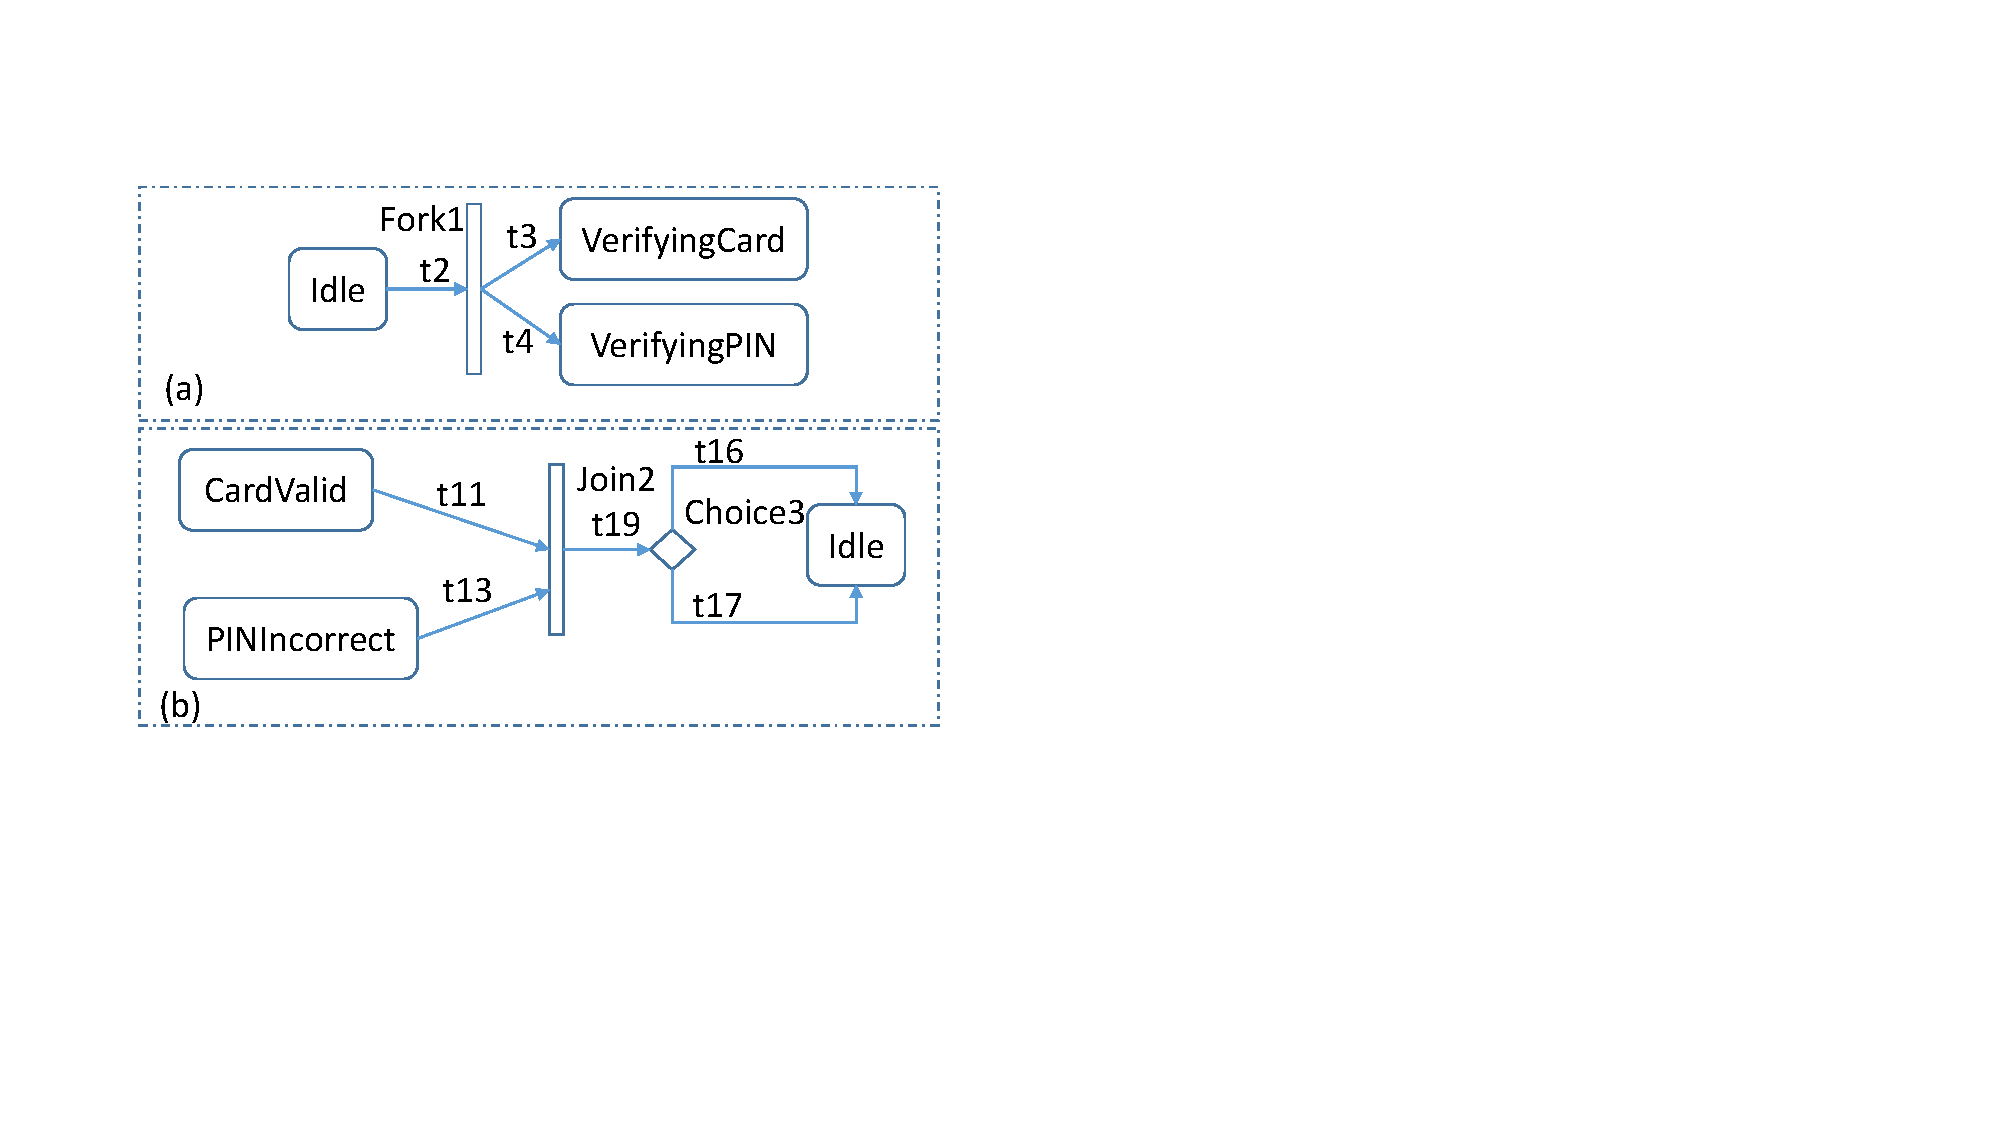
\includegraphics[clip, trim=2.0cm 6cm 17.5cm 3cm, width=\columnwidth]{figures/transitionGraph.pdf}
	\caption{Transition graphs} 
	\label{fig:transitionGraph}
\end{figure}


\begin{definition} A compound transition $t_{cp}$ is a virtual path which starts from one or multiple UML state and ends on one or multiple UML state. A compound transition is specified by a triple \{srcs($t_{cp}$), trc($t_{cp}$), tgts($t_{cp}$)\}, in which source part srcs($t_{cp}$) consists of one or multiple states, transition part trc($t_{cp}$) consists of multiple transitions, and target part tgts($t_{cp}$) consists of one or multiple states. 
\end{definition}


Given a state, Algorithm \ref{alg:cptransition} presents how to calculate transition graphs whose source $t_{cp}$ whose source part contains only a state $s$. 

\begin{algorithm}[]
	\caption{Transition graphs calculation
		\label{alg:cptransition}}
	\begin{algorithmic}[1]
		\Require{A state $s$ of a state machine}
		\Ensure{A set of transition graphs $\mathcal{GT}$}
		\Procedure{calculateTransGraphs}{$s$}
		\Let{$\mathcal{GT}$}{$\emptyset$} 
		\For {$out \in T_{outs}(s)$}
			\If {$tgt(out)$ is not a state}
				\Let{$\tau$}{($\mathcal{S}$, $\mathcal{L}$, $\mathcal{P}$, $\mathcal{T}$) $=\{\emptyset,\emptyset, \emptyset, \emptyset\}$}
				\Let{$\mathcal{P}$}{$\mathcal{P} \cup {tgt(out)}$}
				\Let{$\mathcal{S}$}{$\mathcal{S} \cup \{s\}$}
				\Let{$\mathcal{T}$}{$\mathcal{T} \cup {out}$}
				\If {$tgt(out).kind = join$}
					\Let{$ins$}{\\$\{i \in T_{ins}(tgt(out))| owner(src(i)) = owner(s)\}$}
					\Let{$\mathcal{S}$}{$\mathcal{S} \cup \{src(i)|i \in ins\}$}
					\Let{$\mathcal{T}$}{$\mathcal{T} \cup ins$}
				\EndIf
				\Let{$nexts$}{$FINDTRANS(tgt(out))$}
				\Let{$\mathcal{T}$}{$\mathcal{T} \cup nexts$}
				\Let{H}{\\$\{tgt(t)|t \in nexts \wedge tgt(t).kind = history\}$}
				\Let{$\mathcal{P}$}{$\mathcal{P} \cup \{src(t)|t \in nexts\} \cup H$}
				\Let{$\mathcal{L}$}{$\mathcal{L} \cup \{tgt(t)|t \in nexts \wedge tgt(t)$ is state $\}$}
								
				\Let{$\mathcal{GT}$}{$\mathcal{GT} \cup \{\tau\}$} 
			\EndIf
		\EndFor
		\EndProcedure
		
		\Require{A vertex $v$}
		\Ensure{Transition paths starting from $v$ and ending on a state}
		\Procedure{FindTrans}{$v$}
		\Let{$nextTrans$}{$T_{outs}(v)$}
		\For {$out \in T_{outs}(v)$}
			\If {$tgt(out)$ is not a state}
				\Let {$nextTrans$}{\\$nextTrans \cup FINDTRANS(tgt(out))$}
			\EndIf
		\EndFor	 			 	
		\Return {$nextTrans$} 
		\EndProcedure	
	\end{algorithmic}
\end{algorithm}

For example, applying this algorithm to all states of the state machine example in \ref{fig:example}, we can calculate other transition graphs which are:
\begin{IEEEeqnarray*}{lCr}
	\tau_{3} &=& (\mathcal{S}_3, \mathcal{L}_3, \mathcal{P}_3, \mathcal{T}_3) = (\{VerifyingCard\}, \{Idle, \\ 
	&& {} CardValid\}, \{Choice1\}, \{t5, t6, t7\}),
\end{IEEEeqnarray*}
\begin{IEEEeqnarray*}{lCr}	
	\tau_{4} &=& (\{VerifyingPIN\}, \{PINIncorrect, \\
	&& {} PINCorrect\}, \{Choice2\}, \{t8, t9, t10\}),
\end{IEEEeqnarray*} 
and
\begin{IEEEeqnarray*}{lCr}	
	\tau_{5} &=& (\{CardValid, PINCorrect\}, \{DispenseMoney\}, \\ 
	&& {} \{Join2\}, \{t12, t14, t15\}).
\end{IEEEeqnarray*} 

\end{comment}

\begin{comment}
\begin{definition} A transition graph $\tau$ is an acyclic directed graph ($\mathcal{T}_r$, $\mathcal{P}$, $\mathcal{T}$) where $\mathcal{P}$ is a set of vertexes, and $\mathcal{T}_{r}$ and $\mathcal{T}$ are sets of transitions. $\mathcal{T}_{r}$ is called the set of root transitions of the graph. Following conditions are satisfied:
	\begin{itemize}
		\item $\forall t \in \mathcal{T}_r, src(t)$ is a state.
		
		\item $\forall p \in \mathcal{P}, p.kind \notin \{state, comp, conc\}$.	
		
		\item $\forall t \in \mathcal{T}, src(t)$ is a pseudo state.
	\end{itemize}	
\end{definition}

A traversal from the root transitions of a transition graph to a stable state configuration is a compound transition. A state machine can contain multiple transition graphs. Fig. \ref{fig:transitionGraph} (a) and (b) show two transition graphs $\tau_{1}$ and $\tau_{2}$ of the ATM state machine, respectively, in which 
\begin{IEEEeqnarray*}{lCr}
	\tau_{1} &=& (\mathcal{T}_r, \mathcal{P}, \mathcal{T}) = (\{t2\}, \{Fork1\}, \{t3, t4\} )
\end{IEEEeqnarray*}
and
\begin{IEEEeqnarray*}{lCr}	
	\tau_{2} &=& (\{t11, t13\}, \{Join2, Choice3\}, \{t19, t16, t17\}).
\end{IEEEeqnarray*}



\begin{figure}
	\centering
	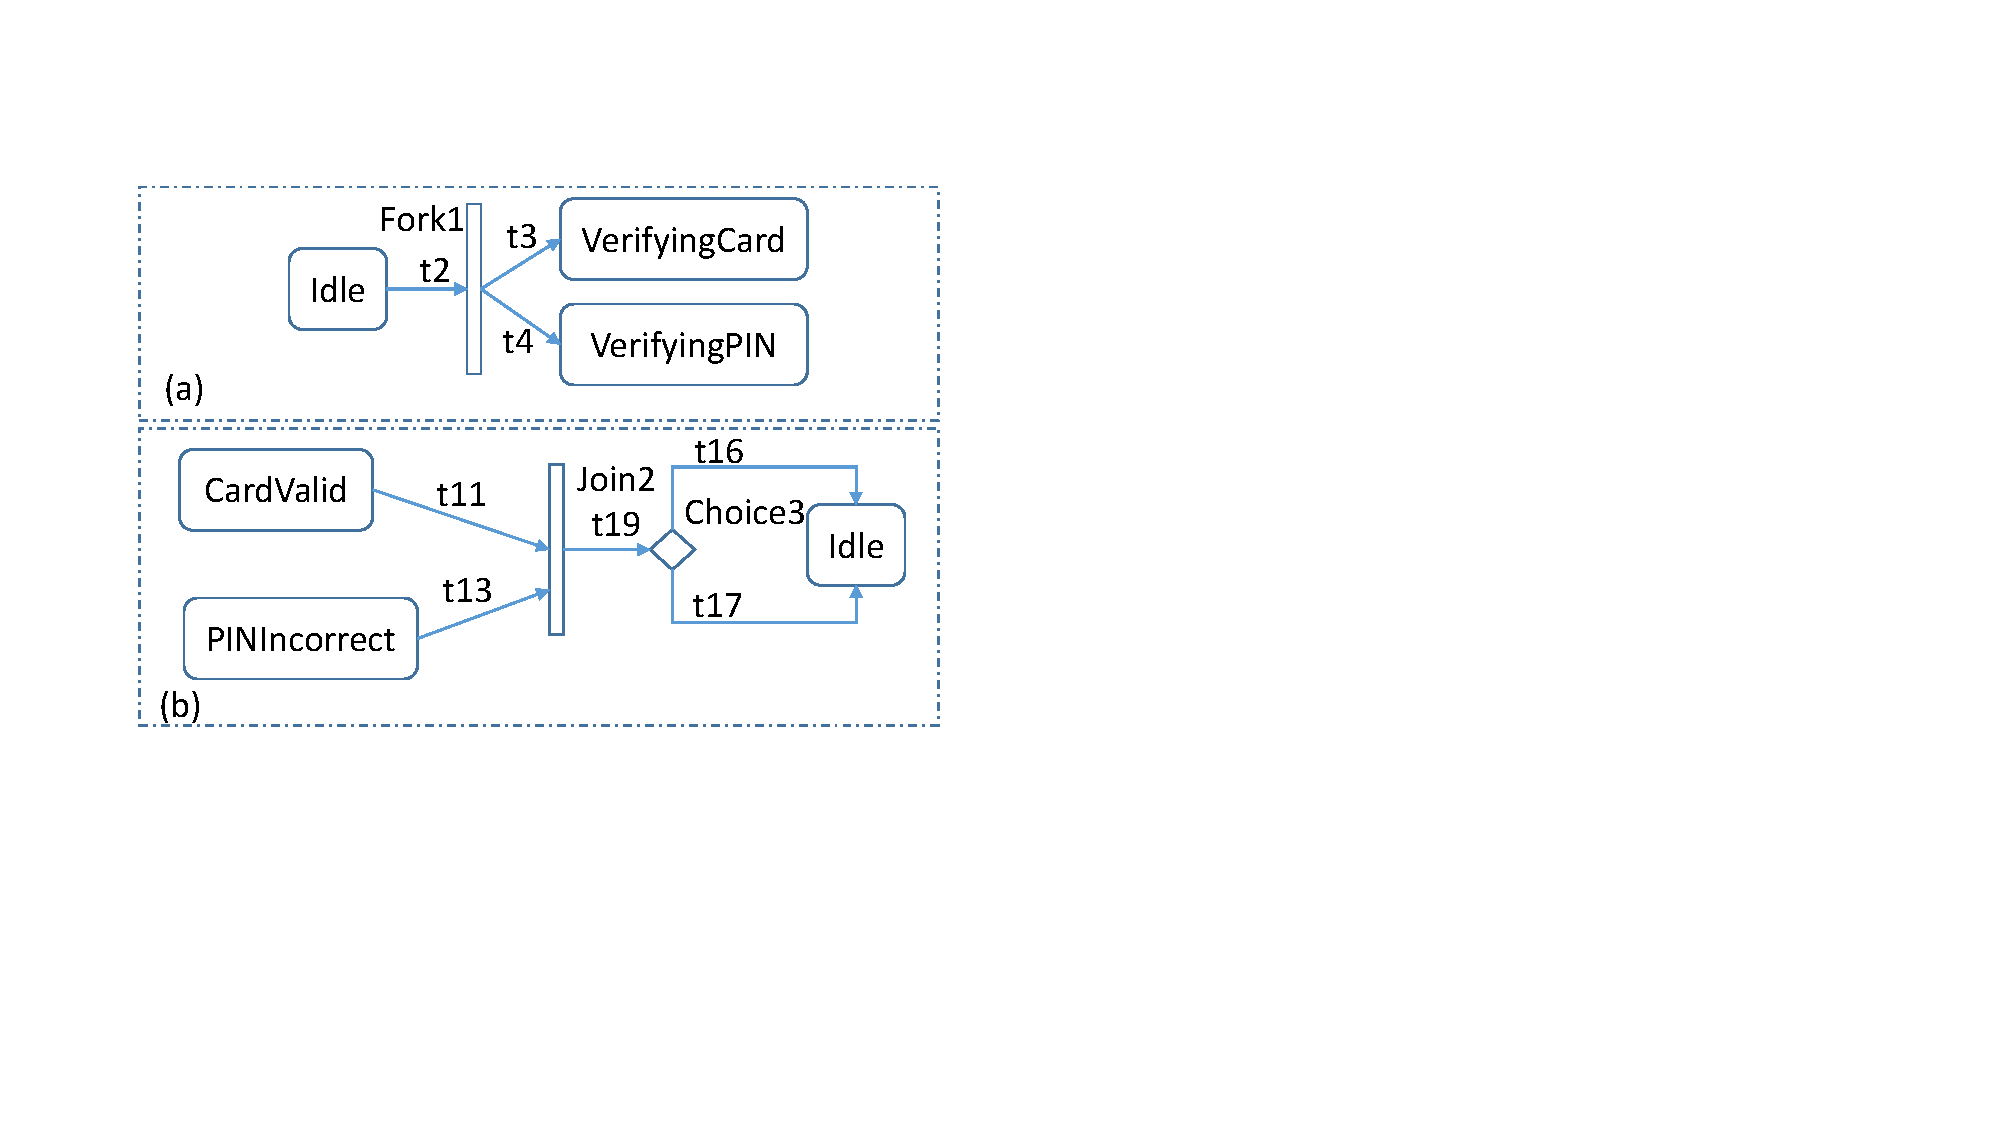
\includegraphics[clip, trim=2.0cm 6cm 17.5cm 3cm, width=\columnwidth]{figures/transitionGraph.pdf}
	\caption{Transition graphs} 
	\label{fig:transitionGraph}
\end{figure}



Given a state, Algorithm \ref{alg:cptransition} presents how to calculate transition graph set whose root transitions outgo from $s$. 

\begin{algorithm}[]
	\caption{Transition graphs calculation
		\label{alg:cptransition}}
	\begin{algorithmic}[1]
		\Require{A state $s$ of a state machine}
		\Ensure{A set of transition graphs $\mathcal{GT}$}
		\Procedure{calculateTransGraphs}{$s$}
		\Let{$\mathcal{GT}$}{$\emptyset$} 
		\For {$out \in T_{outs}(s)$}
			\If {$tgt(out)$ is not a state}
				\Let{$\tau$}{($\mathcal{T}_r$, $\mathcal{P}$, $\mathcal{T}$) $=\{\emptyset,\emptyset, \emptyset\}$}
				\Let{$\mathcal{P}$}{$\mathcal{P} \cup {tgt(out)}$}
				\Let{$\mathcal{T}_r$}{$\mathcal{T}_r \cup {out}$}
			\If {$tgt(out).kind = join$} 
				\Let{$\mathcal{T}_r$}{$\mathcal{T}_r \cup T_{ins}(tgt(out))$}
			\EndIf
				\Let{$nexts$}{$FINDTRS(tgt(out))$}
				\Let{$\mathcal{T}$}{$\mathcal{T} \cup nexts$}
			
				\Let{$\mathcal{GT}$}{$\mathcal{GT} \cup \{\tau\}$} 
			\EndIf
		\EndFor
		\EndProcedure
		
		\Require{A vertex $v$}
		\Ensure{Transition paths starting from $v$ to atomic  states}
		\Procedure{FINDTRS}{$v$}
		\Let{$outs$}{$T_{outs}(v)$}
		\For {$out \in T_{outs}(v)$}
			\If {$tgt(out)$ is not a state}
				\Let {$outs$}{\\$outs \cup FINDTRS(tgt(out))$}
			\ElsIf $tgt(out).kind \in {comp, conc}$
				\For {$sub \in subvertexes(tgt(out)), sub.kind=initial$}
					\Let {$outs$}{$outs \cup FINDTRS(sub)$}
				\EndFor
			\EndIf 
		\EndFor	 			 	
		\Return {$outs$} 
		\EndProcedure	
	\end{algorithmic}
\end{algorithm}

For example, applying this algorithm to all states of the state machine example in \ref{fig:example}, we can calculate other transition graphs which are:
\begin{IEEEeqnarray*}{lCr}
	\tau_{3} &=& (\mathcal{S}_3, \mathcal{L}_3, \mathcal{P}_3, \mathcal{T}_3) = (\{VerifyingCard\}, \{Idle, \\ 
	&& {} CardValid\}, \{Choice1\}, \{t5, t6, t7\}),
\end{IEEEeqnarray*}
\begin{IEEEeqnarray*}{lCr}	
	\tau_{4} &=& (\{VerifyingPIN\}, \{PINIncorrect, \\
	&& {} PINCorrect\}, \{Choice2\}, \{t8, t9, t10\}),
\end{IEEEeqnarray*} 
and
\begin{IEEEeqnarray*}{lCr}	
	\tau_{5} &=& (\{CardValid, PINCorrect\}, \{DispenseMoney\}, \\ 
	&& {} \{Join2\}, \{t12, t14, t15\}).
\end{IEEEeqnarray*} 

\end{comment}
\begin{definition} Current active configuration $Cfg$ of a UML state machine sm is a set of candidate UML states which are able to process an incoming event. 
\end{definition}







\begin{comment}
\section{Thread-based Concurrency}
\label{sec:thread}
\subsection{Thread-based concurrency analysis} 

While concurrency is an important aspect defined by the UML State machine specification, especially hierarchical and concurrent state machines with \ti{doActivity}s for states, most of existing approaches do not take into account. This is non-trivial since concurrency is dynamic in UML state machine since the number of threads used for concurrency is non-deterministic.

Let us give an analysis on the state machine example in Fig. \ref{fig:example}. Assuming that \ti{Idle} is the current active state and a \ti{verifyPIN} event is coming. 
The \ti{doActivity} behavior of \ti{Idle} \ti{doActivity(Idle)} (if has) is terminated, \ti{exit(Idle)} and the \ti{effect(t2)} (\ti{T2Effect}) are executed sequentially. 
These actions are run in a state machine main thread which reads incoming events from a "first in, first out" (FIFO) priority queue. 
Fig. \ref{fig:threading1} shows the activity diagram representing the concurrency processing \ti{verifyPIN}, in which each partition represents a thread. 
\ti{effect(t3)} and \ti{effect(t3)} are run concurrently in two threads \ti{T3Run} and \ti{T4Run}, respectively, since the transitions owning these effects outgo from a fork pseudo state. 
The entry action \ti{entry(Verifying)} is executed following the termination of the two threads. 

UML says that \ti{doActivity(Verifying)}, \ti{entry(VerifyingCard)} and \ti{entry(VerifyingPIN)} should be concurrently executed upon the completion of \ti{entry(Verifying)}, which is represented by a fork node, in which a \ti{Start} signal is sent to \ti{VerifyingDoRun} in order for commencing \ti{doActivity(Verifying)}. 
The executions of the \ti{doActivity}s of the states \ti{VerifyingCard} and \ti{VerifyingPIN} are also concurrent. 
Also, upon the completion of \ti{entry(VerifyingCard)} and \ti{entry(VerifyingPIN)}, the main thread completes the processing of the \ti{verifyPIN} event, reads next events from the queue or waits for next event occurrences.

\begin{figure}
	\centering
	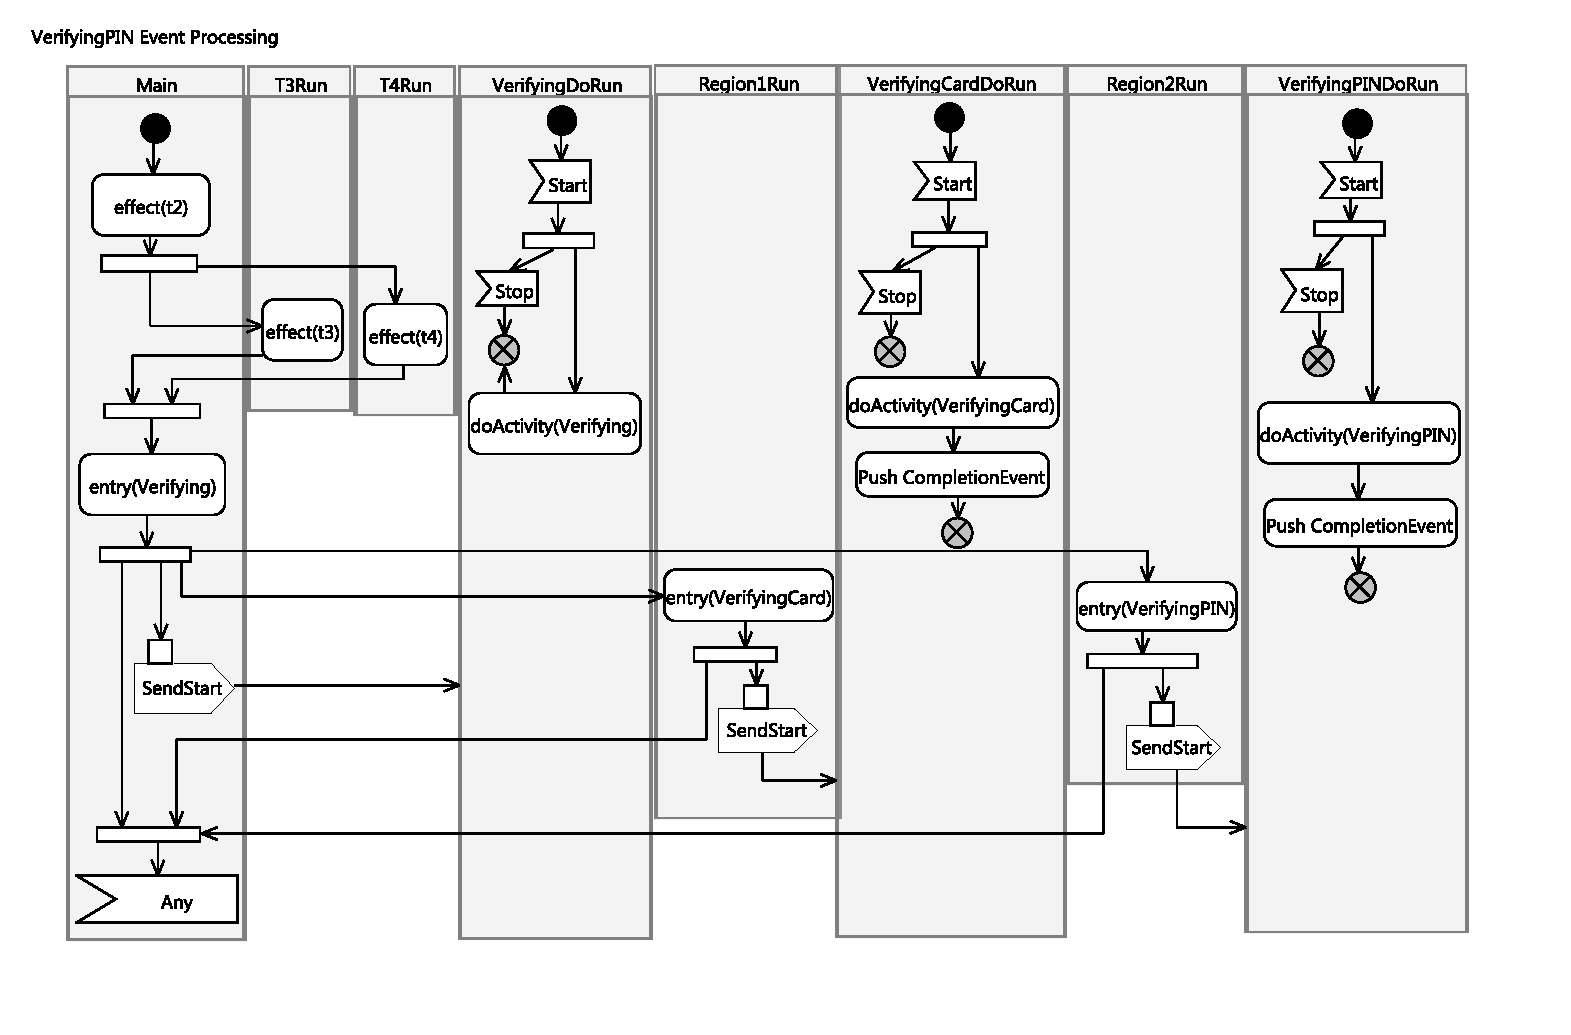
\includegraphics[clip, trim=1.0cm 1.6cm 1.6cm 1cm, width=1.03\columnwidth]{figures/ThreadingExample.pdf}
	\caption{Concurrency of the ATM when receiving the \ti{verifyingPIN} event} 
	\label{fig:threading1}
\end{figure}

If no event is coming, and \ti{doActivity(VerifyingCard)} and \ti{doActivity(VerifyingPIN)} are long actions (e.g. forever loops inside), the state machine remains its active configuration and three concurrent actions including \ti{CheckForEvents}, \ti{doActivity(VerifyingCard)}, and \ti{doActivity(VerifyingPIN)} are permanently run.

The termination time of \ti{doActivity(VerifyingCard)} and \ti{doActivity(VerifyingPIN)} is non-deterministic. 
However, a completion event is generated and pushed to the event queue whenever one of the two completes. 
For illustration, assuming that \ti{doActivity(VerifyingCard)} terminates before \ti{doActivity(VerifyingPIN)}. 
As in Fig. \ref{fig:threading2}, the Main thread checks the \ti{CompletionEvent}. \ti{exit(VerifyingCard)} and \ti{effect(t5)} are then executed sequentially. If \ti{cardValid} is computed as true as the result of \ti{doActivity(VerifyingCard)} and \ti{exit(VerifyingCard)}, the Main thread simply executes \ti{effect(t6)} and \ti{entry(CardValid)} before waiting for other events.

In contrast, Main sends a signal to stop \ti{doActivity(VerifyingPIN)} and \ti{doActivity(Verifying)}, executes exit, transition and entry actions in an appropriate order (see Fig. \ref{fig:threading2}) and waits for other events.

We see that the number of concurrent actions is not constant but changes timely. 
Each action can either deterministically or non-deterministically terminate. 
In this sense, deterministic actions (DAs) prevent the Main thread from going to the waiting-for-event point. 
In other words, pending events in the queue are only read and processed once all deterministic actions complete. Therefore, we re-define the run-to-completion paradigm of UML state machine as following:
 
\begin{definition}
	Run-to-completion means that, in the absence of exceptions or asynchronous destruction of the context	class object or the state machine execution, a pending Event occurrence is dispatched only after the completion of all deterministic actions commenced by the processing of the current event. 
	At this point, a stable state configuration has been reached
\end{definition}

In the example, some of DAs are as followings: \ti{effect(t2)}, \ti{effect(t4)}, \ti{entry(Verifying)}, \ti{entry(VerifyingCard)}, and non-deterministic actions (NDAs) as followings: \ti{doActivity(Verifying)}, \ti{doActivity(VerifyingCard)} and \ti{doActivity(VerifyingPIN)}.


\begin{figure}
	\centering
	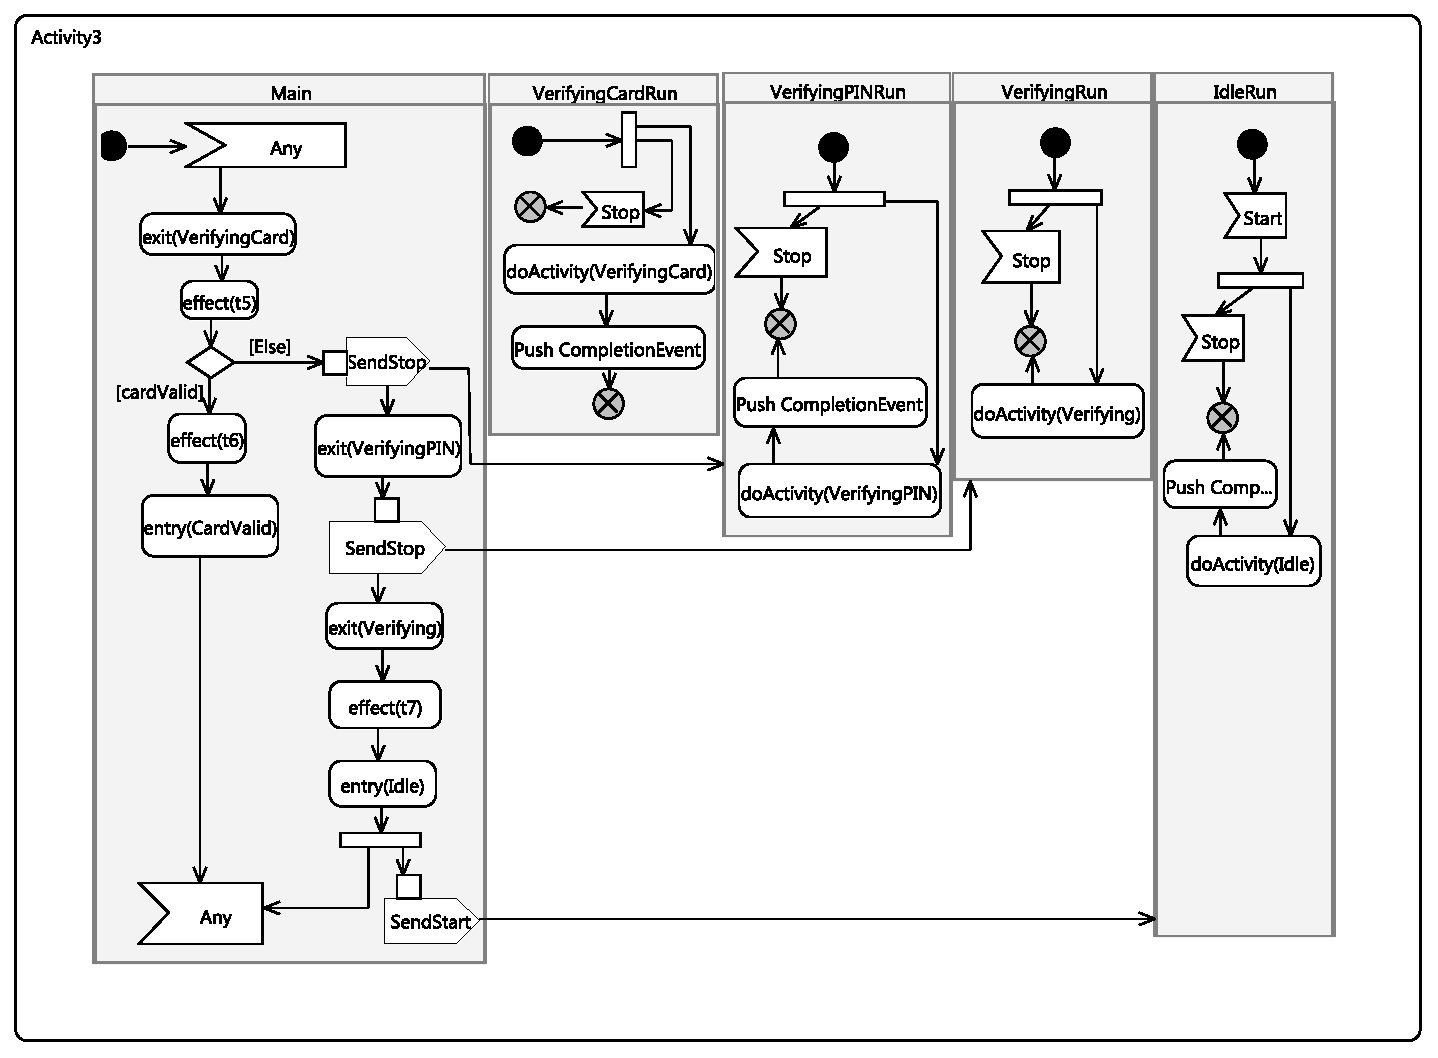
\includegraphics[clip, trim=1.5cm 1.6cm 1.6cm 1.2cm, width=1.03\columnwidth]{figures/ThreadingExample2.pdf}
	\caption{Concurrency of the ATM when \ti{doActivity} of \ti{VerifyingCard} completes before that of \ti{VerifyingPIN}}
	\label{fig:threading2}
\end{figure}

\subsection{Thread-based design of generated code}
Each NDA is run in parallel with the main thread which reads and dispatch events from the event queue. 
Each is associated with a thread which is initialized at the state machine initialization moment. 
The number of threads associated with NDAs is therefore equal to that of the NDAs.
The design of threads is based on the thread pool pattern, which initializes all threads at once, and the paradigm "wait-execute-wait". 
In the latter, a thread \tb{waits} for a signal to \tb{execute} its associated method and goes back to the \tb{wait} point if it receives a stop signal or its associated method completes. 
An NDA is one of the followings:
\begin{itemize}
	\item \ti{doActivity} of each state if has. The number of \ti{doActivity} $n_{do} = \#\{s \in V|\exists doActivity(s)\}$
	
	\item Sleep function associated with a \ti{TimeEvent} which counts ticks and emits a \ti{TimeEvent} once completes: $n_{te} = \#\{e \in E|\ti{e is a time event}\}$.
	
	\item Change detect function associated with a \ti{ChangeEvent} which observes a variable or a boolean expression and pushes an event to the queue if changes happen: $n_{che} = \#\{e \in E|\ti{e is a change event}\}$.
\end{itemize} 

Therefore, the concurrency has the number of initial threads $n_{threads} = n_{do} + n_{te} + n_{che}$ plus a main thread which reads events from the event queue, and sends start and stop signals to these initial threads. 

Now we consider spontaneous threads which are created to run DAs, joined until and destroyed once DAs complete. 
\end{comment}
\begin{comment}
The followings describe different types of DAs:

\begin{itemize}
	\item Actions executed when entering/exiting an orthogonal region, which can be: execute a chain of transition effects contained by the region before entering a stable sub-state or exiting the region completely.%: $n_{region threads} = \#\{r \in \mathcal{R}|ctner(r).kind=conc\}$
	
	\item Effects of transitions outgoing from a $fork$ and those incomings to a $join$.%: \\
	%$\mathcal{J} = \{v \in V|v.kind=join\}$ \\
	%$\mathcal{F} = \{v \in V|v.kind=fork\}$ \\
	%$$n_{FJ\_threads} = \sum_{v \in \mathcal{F}} {\#T_{outs}(v)} + \sum_{v \in \mathcal{J}} {\#T_{ins}(v)}$$.
\end{itemize}
%\end{comment}
\begin{comment}
The spontaneous threads follow a paradigm in which if a thread $parent$ creates a set of threads $children$, $parent$ must wait until $children$ complete their associate methods. These threads are created in one of the following cases:

\begin{itemize}
	\item A thread is created for each effect of transitions' outgoing from a \ti{fork} or incoming to a \ti{join}.
	
	\item Entering a concurrent state $s$, after the execution of $entry(s)$, a thread is also created for each orthogonal region. 
	
	\item Exiting a concurrent state $s$, before the execution of $exit(s)$, a thread is also created for each region to exit the corresponding active sub-state.
	
	\item An event is processed by active states, in which a thread per orthogonal region. 
\end{itemize}

\subsection{Deadlock avoidance}
Each NDA thread is associated with a mutex for synchronization communication in the multi-thread-based generated code. 
The mutex must be locked before the method associated with the thread is executed. 
The mutex associated with the main thread protects the run-to-completion semantics since some event such as \ti{CallEvent} can be processed synchronously and some asynchronously. Each event processing must lock the main mutex before executing the actual processing. 
%Deadlock is one of the main issues in designing multi-thread applications, in which two competing actions wait for the other to finish. In our case, 
\end{comment}

\begin{comment}
\begin{tabular}{p{4.0cm}|p{4.0cm}}
Example code generated for doActivity  &  Option  2\\
\begin{lstlisting}[language=C++]
void doActivity(int stateId) {
  isStarts[stateId] = false;
  while(true) {
    mutex[stateId].lock();
    while(!isStarts[stateId]) {
      mutex[stateId].wait();
    }
    states[stateId].doActivity();
    isStarts[stateId] = false;
    mutex[stateId].unlock();
    if (!isStops[stateId]) {
      if (stateId == IDLE_ID || stateId == DISPENSEMONEY_ID ...) {
	    pushCompletionEvent(stateId);
	  }
    }
  }
}
	\end{lstlisting}&
	\begin{lstlisting}
	#include <stdio.h>
	
	int main()
	{
	printf("Hello world\n");
	}
	\end{lstlisting}
\end{tabular} 
\end{comment}
















\section{\uppercase{Concurrency}}
\label{sec:thread}
This section describes our design of concurrency aspects of state machines in generated code at runtime. 
%The design is based on an example-based analysis, which is not presented here due to space limitation.

%\input{sections/analysis}
\subsection{Thread-based design}
The concurrency of USMs is based on multiple threads including permanent and spontaneous threads. 
While permanent threads (PTs) are created once and live as long as the state machine is alive, spontaneous threads (STs) are spawned and active for a while. 
%The method associated with a permanent thread is a non-deterministic action, which is run in parallel with the main thread. The latter reads and dispatch events from the event queue. 
Each PT is initialized at the state machine initialization. 
%The number of threads associated with NDAs is therefore equal to that of the NDAs.
The design of threads is based on the thread pool pattern, which initializes all threads at once, and the paradigm "wait-execute-wait". 
In the latter, a thread \tb{waits} for a signal to \tb{execute} its associated method and goes back to the \tb{wait} point if it receives a stop signal or its associated method completes. 
Each PT is associated with one of the following actions:

{
\begin{itemize}
	\setlength\itemsep{-0.25em}
	\item \ti{doActivity} of each state if has any. %The number of \ti{doActivity} $n_{do} = \#\{s \in V|\exists doActivity(s)\}$
	
	\item Sleep function associated with a time event which counts ticks and emits the event once completes.%: $n_{te} = \#\{e \in E|\ti{e is a time event}\}$.
	
	\item Change detect function associated with a change event which observes a variable or a boolean expression and pushes an event to the queue if a change occurs.%: $n_{che} = \#\{e \in E|\ti{e is a change event}\}$.
	
	\item State machine main thread, which reads events from the event queue, and sends start and stop signals to other PTs.
\end{itemize} 
}

%Therefore, The number of initial threads is $n_{threads} = n_{do} + n_{te} + n_{che}$ plus a main thread, which reads events from the event queue, and sends start and stop signals to these initial threads. 

STs which are spawned by a parent thread, joined until and destroyed once the associated methods complete. 
\begin{comment}
The followings describe different types of DAs:
\begin{itemize}
\item Actions executed when entering/exiting an orthogonal region, which can be: execute a chain of transition effects contained by the region before entering a stable sub-state or exiting the region completely.%: $n_{region threads} = \#\{r \in \mathcal{R}|ctner(r).kind=conc\}$

\item Effects of transitions outgoing from a $fork$ and those incomings to a $join$.%: \\
%$\mathcal{J} = \{v \in V|v.kind=join\}$ \\
%$\mathcal{F} = \{v \in V|v.kind=fork\}$ \\
%$$n_{FJ\_threads} = \sum_{v \in \mathcal{F}} {\#T_{outs}(v)} + \sum_{v \in \mathcal{J}} {\#T_{ins}(v)}$$.
\end{itemize}
\end{comment}
The STs follow a paradigm in which the spawning parent must wait until its children complete their associated methods. These threads are used for the following cases:

{
\begin{itemize}
	\setlength\itemsep{-0.25em}
	\item A thread is created for each effect of transitions outgoing from a \ti{fork} or incoming to a \ti{join}.
	
	\item Entering a concurrent state, after the entry action of the state, a thread is created for each orthogonal region. 
	
	\item Exiting a concurrent state, before the exit action of the state, a thread is created for each region to exit the corresponding active sub-state.
	
	%\item An event is processed by active states, in which a thread per orthogonal region. 
\end{itemize}
}
\subsection{Thread communication}
\label{subsec:deadlock}
Each PT is associated with a mutex for synchronization in the multi-thread-based generated code. 
The mutex must be locked before the method associated with the thread is executed. 


\vskip 0.1cm
\noindent
\tb{Run-to-completion:} The event process must follow the run-to-completion semantics of UML State Machines.
The semantics means that the state machine completes processing of each event before starting processing the next event. 
If all events are asynchronous, the main thread processes events by reading one-by-one from the event queue.
However, because we allow call events to be synchronous, the processing of synchronous and asynchronous events can violate the run-to-completion semantics.
To avoid it, a main mutex is associated with the main thread to protect the run-to-completion semantics. 
Each event processing must lock the main mutex before executing the actual processing. 
%Deadlock is one of the main issues in designing multi-thread applications, in which two competing actions wait for the other to finish. In our case, 
In generated code, lock and unlock are implemented using signals and conditions in POSIX \cite{Posix}.

%\vskip 0.1cm
\noindent
%\tb{Multi-threaded problems checking:}
%We use POSIX threads to realize concurrency in UML State Machines.
%We use the Valgrind DRD tool \cite{DRD} to check multi-thread problems such as data races, deadlock, and misuse of POSIX threads API in generated code derived from the PSSM test suite.
%The generated code is free of multi-thread errors.
%The result shows that code generated by our tool potentially avoids multi-thread problems. 

\begin{comment}
\begin{tabular}{p{4.0cm}|p{4.0cm}}
Example code generated for doActivity  &  Option  2\\
\begin{lstlisting}[language=C++]
void doActivity(int stateId) {
isStarts[stateId] = false;
while(true) {
mutex[stateId].lock();
while(!isStarts[stateId]) {
mutex[stateId].wait();
}
states[stateId].doActivity();
isStarts[stateId] = false;
mutex[stateId].unlock();
if (!isStops[stateId]) {
if (stateId == IDLE_ID || stateId == DISPENSEMONEY_ID ...) {
pushCompletionEvent(stateId);
}
}
}
}
\end{lstlisting}&
\begin{lstlisting}
#include <stdio.h>

int main()
{
printf("Hello world\n");
}
\end{lstlisting}
\end{tabular} 
\end{comment}



\section{Code generation}
%\subsection{Transformation pattern}
%todo: describe the pattern

%Transformation from State machine to fUML (classes, attributes, methods)
%\lipsum[1]

\subsection{Assumption}
%todo: give some assumptions on code generation such as functions to create methods, attriutes, classes
To give the formalization of the code generation, we assume that we want to generate from the state machine to an object oriented programming language $ActLang$. Assuming that our code generator contains primitive functions supporting for generating $ActLang$ as following:
\begin{itemize}
	\item $genClass(n, generals, itfs)$ creates a class with its name, parent class set, and implemented interfaces as \ti{n}, \ti{generals}, and \ti{itfs}.
	
	\item $genMtd(n, c, type, params)$ creates a method $m$ with its name as $n$ inside the class $c$, its return type as $type$, and $params$ as its parameter set.
	
	\item $genAttr(n, c, type, multiplicity)$ creates an attribute named $n$ in the class $c$ and typed by $type$. The create attribute is an array if $multiplicity > 1$, otherwise a simple attribute.
	
	\item $genEnum(n)$ and $genEnumLit(enum, n)$ create an enumeration and its enumeration literal, respectively.
	
	\item $genBody(m, body)$ adds a body to a method. The body is a string which contains a list of statements.
	
	\item $createParalle(t, seg)$ generates a mechanism which allows the segment code $seg$ run in a thread $t$. Similarly, $genWait(t), genJoin(t)$.
	
	\item $genMutex(size)$ creates an array of mutexes with \ti{size} as the number of items of the array. 
	
	\item $synchronize(seg)$ generates a mechanism which allows the segment code $seg$ run safely (can be either based on \ti{POSIX pthread} or \ti{Java synchronize} mechanism).
	
	\item $toString(stts)$ is used to convert a list of statements $stts$ into a readable string which can be add to a method as its body.
	
	\item Concatenation of two strings $str1$ and $str2$ is concisely described as $str1 + str2$.
	
	\item \ti{WHILE}, \ti{FOR} \ti{IF}, \ti{ELSE} are symbols representing while and for loops, if and else statements.
	
	\item \ti{FORK(func)} creates a thread (lightweight process) associated with the function/method \ti{func} and \ti{JOIN(theThread)} waits until the method associated with the thread \ti{theThread} completes.
\end{itemize} 

\subsection{Code generation algorithm}
\subsubsection{State transformation}
Suppose that we want to generate a state machine $sm$ whose states are listed by $lstates$. A common state interface $IState$ is created. The interface contains three methods, namely, \ti{entry}, \ti{exit}, and \ti{doActivity} corresponding to three state actions, respectively. To preserve the hierarchy of composite states, the interface also has two attributes called \ti{activeStates} and \ti{previousStates} referring to active sub-states \ti{actives} , previous active sub-states \ti{previousStates} in case of the presence of history states, and a list of deferred event identifiers.

Each UML state is transformed into an instance of the interface associated with a state ID (which is a child element of an enumeration) inside the active class $C$. When initialization, each instance refers its methods to the actual methods implemented in $C$. In C++, this referring is done by using the powerful mechanism function pointer. In other object-oriented languages such as Java, this is done with anonymous sub-classes of the interface. Listing \ref{lst:IStateCpp} and \ref{lst:IStateJava} show the interface and its instances associated with the states of the state machine in C++ and Java, respectively, in which S0 is one of $lstates$. \ti{NUM\_STATES} is the number of states in the state machine. The actions of the states are implemented in the active class $C$ and named depending on the name of the states. In the following sections, we only consider C++ as out \ti{ActLang}. The discussion of other object-oriented languages are much similar since these share the same concepts,  

\begin{lstlisting}[caption=IState interface and function pointers in C++, label=lst:IStateCpp, frame=single]
typedef struct IState {
  IState** previousStates; 
  IState** actives;
  EventId* defEvents;
  void (C::*entry)();
  void (C::*exit)();
  void (C::*doActivity)();
} IState;
class C {
private:
  IState states[NUM_STATES];
public:
  C() {
    states[S0_ID].entry = &C::S0_entry;
    ...
  }
  void S0_entry {...}
}
\end{lstlisting}

\begin{lstlisting}[mathescape=true, caption=IState interface and annonymous sub-classes in Java, label=lst:IStateJava, frame=single]
public interface IState {
  public IState[] previousStates; 
  public IState[] actives;
  public EventId defEvents;
  public void entry();
  public void exit();
  public void doActivity();
}
class C {
private IState states[NUM_STATES];
public C() {
  states[S0_ID] = new IState() {
    public void entry() {
      S0_entry();
    }
    ...
  }
}
public void S0_entry() {...}
}
\end{lstlisting}

The procedure to generate the code for states is shown in Listing \ref{lst:procedure1}. It first creates the state interface $IState$ (in C++, it is either a class or a struct). The array attribute is then created with the number of states as its size. Each state is also associated with a state ID which is a child of an enumeration. Finally, the constructor of $C$ is created to initialize and make methods of the attribute instances refer to \ti{entry/exit/doActivity} action methods of $C$. The implementation of action methods in the context class $C$ is similar to the delegation pattern proposed by the authors in \cite{Niaz2004} but dramatically decreases the memory consumption since only one common interface for all states is created instead of a class for each state in \cite{Niaz2004}.

\begin{lstlisting}[mathescape=true, caption=Procedure to create code for states, label=lst:procedure1, frame=single]
IState = genClass('IState', $\emptyset$, $\emptyset$);
stateIdEnum = genEnum('StateIdEnum');
foreach s in lstates
  genEnumLit(stateIdEnum, s.name + '_ID');
  mtd = genMtd(s.name + '_entry', C, 
			null, null);
  genBody(mtd, toString(entry(s)));
  ...
genEnumLit(stateIdEnum, 'NUM_STATES');  
genAttr('states', C, IState, NUM_STATES); 
genMtd(C.name, C, null, null);
\end{lstlisting}

\subsubsection{Region transformation}


\subsubsection{Event transformation}
An event enumeration \ti{EventId} is created whose children are event identifiers associated with events. Each event is also transformed into a method in the context class $C$. Suppose $levents$ is the list of events which can be processed by the state machine $sm$. Besides the explicitly defined events of the state machines, $levents$ contains a special event called $CompletionEvent$. The latter is, following the UML specification, an implicit event triggering triggerless transitions. It is emitted when either \ti{doActivity} of an atomic state finishes its execution or all orthogonal regions of a composite state have reached to a final state. 

UML defines five types of events including \ti{CallEvent}, \ti{SignalEvent}, \ti{TimeEvent}, \ti{ChangeEvent}, and \ti{Any}. A transition triggered by an \ti{Any} event is meant to be fired by any of the other events. To process events, for each event, a method is implemented in $C$. Each event triggers a list of transitions. We suppose $T_{trig}(e)$ is the transition list triggered by the event $e$, and $S_{trig}(e) = \{src(t) | t \in T_{trig}(e)\}$. In other words, $S_{trig(e)}$ is a set of states which are the source states of the transitions in $T_{trig}(e)$. To present how the body of event methods is generated, we define functions as followings:
\begin{itemize}
	\item Vertex depth $dp(v)$ is defined as:
			\begin{equation}
			dp(v) =    \left\{
			\begin{array}{ll}
			1 & \ti{v is a root vertex}  \\
			dp(ctner(v)) + 1& otherwise \\
			\end{array} 
			\right.
			\end{equation}
	\item $Map_{e}(s) \subset S_{trig(e)} | \forall sub \in map_e(s): ctner(sub) = s$, $Prt(e) = \{s \in V| map_{e}(v) \neq \emptyset\}$. $Prt(e)$ is an ordered list whose length is $len(Prt\{e\})$ and elements are accessed by indexes. The order of $Prt(e)$ is defined as:	$\forall i, j \leq len(Prt\{e\})$, 
	\\ if $i < j, dp(Prt(e).get(i)) \geq dp(Prt(e).get(j))$. 	
\end{itemize}


The procedure in Listing \ref{lst:eventproc} describes how to generate the body of the method associated with an event. It generates the code checking for active states respecting the UML semantics in which the innermost states process the incoming event first. To do this, it first looks in the source state list $S_{trig(e)}$ for the innermost states that accept the event triggering its outgoing transitions. If these found states are children of a concurrent state, $genStateCheck$ generates the checking codes run in parallel, which will be described later in \ref{subsubsec:thread}. Otherwise said, sequential code is generated.

\begin{lstlisting}[mathescape=true, caption=Procedure to create code event processing, label=lst:eventproc, frame=single]
for item in $Lm(e)$
  if ($item.kind = conc$)
    for s in Map_e(item)
      genStateCheck() 
  else 
    for s in Map_e(item)
      genStateCheckWithElse  	
\end{lstlisting}



\subsubsection{Thread-based Concurrency}
\label{subsubsec:thread}
\paragraph{Thread-based concurrency analysis} 

While concurrency is an important aspect defined by the UML State machine specification, especially hierarchical and concurrent state machines with \ti{doActivity}s for states, most of existing approaches do not take into account. This is non-trivial since concurrency is dynamic in UML state machine since the number of threads used for concurrency is non-deterministic.

For example, assuming that \ti{Idle} is the current active state of the ATM state machine in Fig. 
\ref{fig:example} and a \ti{verifyPIN} event is coming. 
The \ti{doActivity} behavior of \ti{Idle} \ti{doActivity(Idle)} (if has) is terminated, \ti{exit(Idle)} and the \ti{effect(t2)} (\ti{T2Effect}) are executed sequentially. 
These actions are run in a state machine main thread which reads incoming events from a "first in, first out" (FIFO) priority queue. 
Fig. \ref{fig:threading1} shows the activity diagram representing the concurrency of the state machine example when processing the \ti{verifyPIN} event, in which each activity partition represents a thread. 
The completion of \ti{effect(t2)} is followed by \ti{effect(t3)} and \ti{effect(t3)}, which are run concurrently since the transitions owning these effects outgo from a fork pseudo state. 
Two threads \ti{T3Run} and \ti{T4Run} associated with \ti{effect(t2)} and \ti{effect(t3)}, respectively, are created by \ti{FORK}.
The entry action \ti{entry(Verifying)} of \ti{Verifying} is executed following the termination of the two threads. 

After \ti{entry(Verifying)} completion, the UML specification says that \ti{doActivity(Verifying)}, \ti{entry(VerifyingCard)} and \ti{entry(VerifyingPIN)} should be concurrently executed, which is represented by a fork node, in which a \ti{Start} signal is sent to \ti{VerifyingDoRun} in order for commencing \ti{doActivity(Verifying)}. 
As the \ti{Verifying} state, the \ti{doActivity}s of the states \ti{VerifyingCard} and \ti{VerifyingPIN} are also concurrently started. 
Also, upon the completion of \ti{entry(VerifyingCard)} and \ti{entry(VerifyingPIN)}, the main thread completes the processing of the \ti{verifyPIN} event, reads next events from the queue or waits for next event occurrences.

\begin{figure}
	\centering
	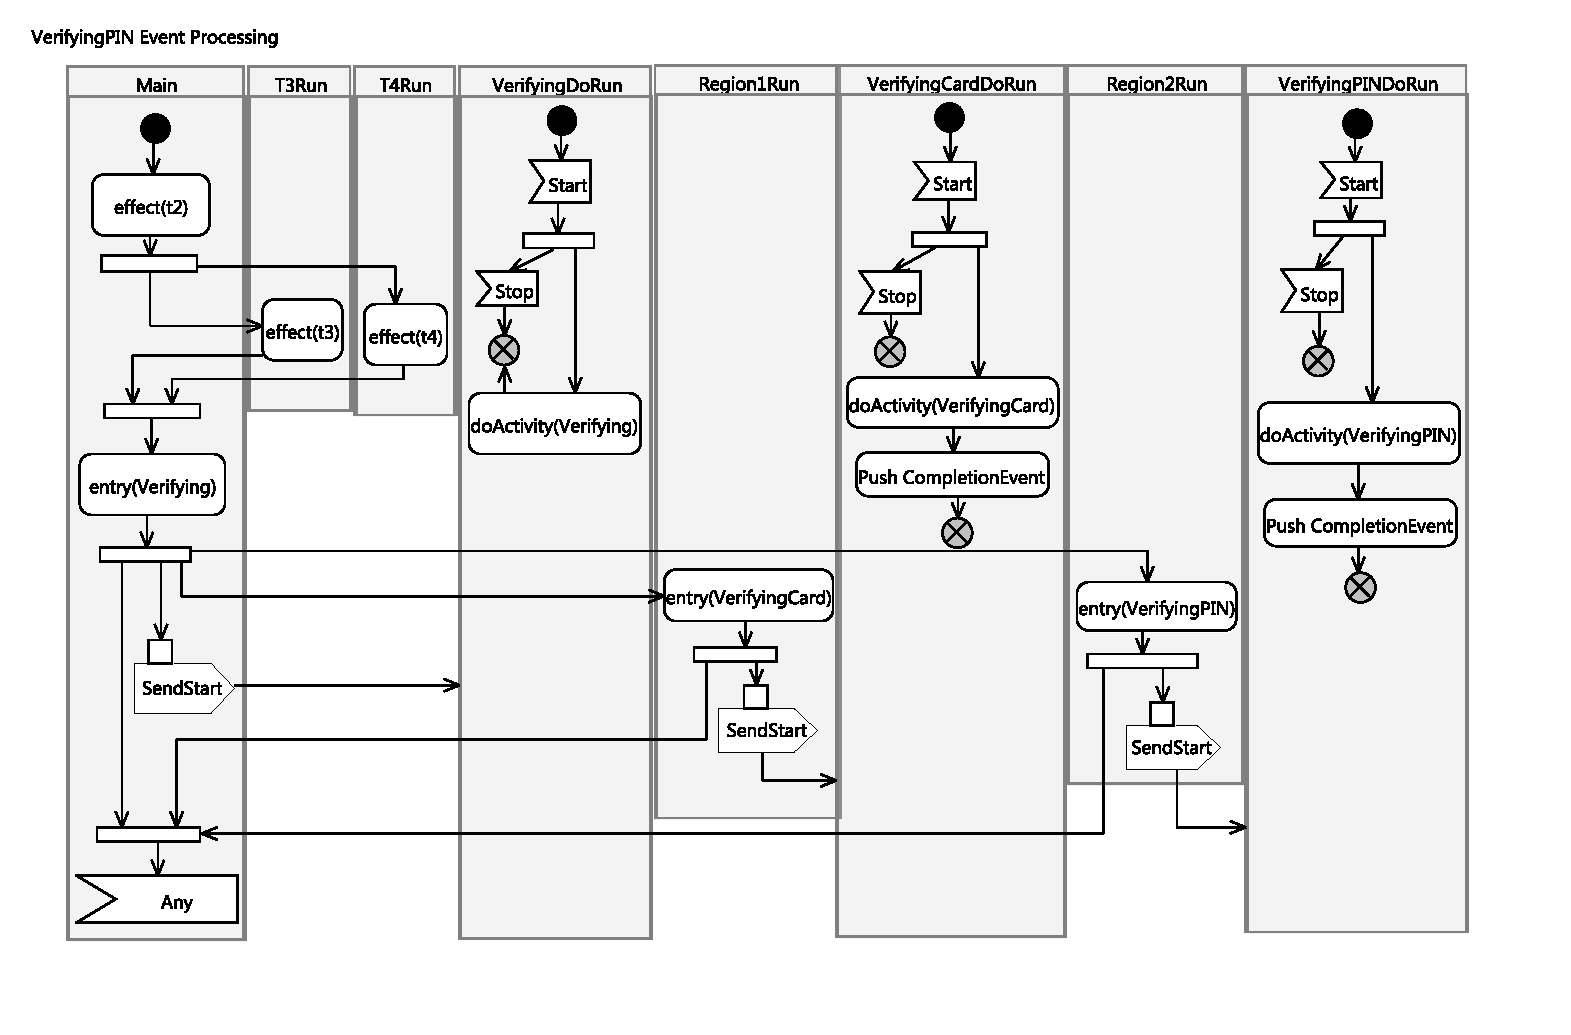
\includegraphics[clip, trim=1.0cm 1.6cm 1.6cm 1cm, width=1.03\columnwidth]{figures/ThreadingExample.pdf}
	\caption{Concurrency of the ATM when receiving the \ti{verifyingPIN} event} 
	\label{fig:threading1}
\end{figure}

If no event is coming, and \ti{doActivity(VerifyingCard)} and \ti{doActivity(VerifyingPIN)} are long actions (e.g. forever loops inside), the state machine remains its active configuration and three concurrent actions including \ti{CheckForEvents}, \ti{doActivity(VerifyingCard)}, and \ti{doActivity(VerifyingPIN)} are permanently run.

It is worth noting that the termination time of \ti{doActivity(VerifyingCard)} and \ti{doActivity(VerifyingPIN)} is non-deterministic. 
However, whenever one of those completes, a completion event associated with the state corresponding to the completed \ti{doActivity} is generated and pushed to the event queue. 
For illustration, assuming that \ti{doActivity(VerifyingCard)} terminates before \ti{doActivity(VerifyingPIN)}. 
As the activity diagram in Fig. \ref{fig:threading2}, the Main thread checks the \ti{CompletionEvent} upon the completion of \ti{doActivity(VerifyingCard)}. \ti{exit(VerifyingCard)} and \ti{effect(t5)} are then executed sequentially. If \ti{cardValid} is computed as true as the result of \ti{doActivity(VerifyingCard)} and \ti{exit(VerifyingCard)}, the Main thread simply executes \ti{effect(t6)} and \ti{entry(CardValid)} before waiting for other events.

In contrast, Main sends \ti{Stop} signals to stop \ti{doActivity(VerifyingPIN)} and \ti{doActivity(Verifying)}, executes exit actions, effects and entry actions in an appropriate order (see Fig. \ref{fig:threading2}) and waits for other events.

So far, we see that the number of concurrent actions is not constant but changes timely. 
Each action can either deterministically or non-deterministically terminate. 
In this sense, deterministic actions (DAs) prevent the Main thread from going to the waiting-for-event point. 
In other words, pending events in the queue are only read and processed once all deterministic actions complete. Therefore, we re-define the run-to-completion paradigm of UML state machine as following:
 
\begin{definition}
	Run-to-completion means that, in the absence of exceptions or asynchronous destruction of the context	class object or the state machine execution, a pending Event occurrence is dispatched only after the completion of all deterministic actions commenced by the processing of the current event. 
	At this point, a stable state configuration has been reached
\end{definition}

In the example, some of DAs are as followings: \ti{effect(t2)}, \ti{effect(t3)}, \ti{effect(t4)}, \ti{entry(Verifying)}, \ti{entry(VerifyingCard)}, \ti{entry(VerifyingPIN)} and non-deterministic actions (NDAs) as followings: \ti{doActivity(Verifying)}, \ti{doActivity(VerifyingCard)} and \ti{doActivity(VerifyingPIN)}.


\begin{figure}
	\centering
	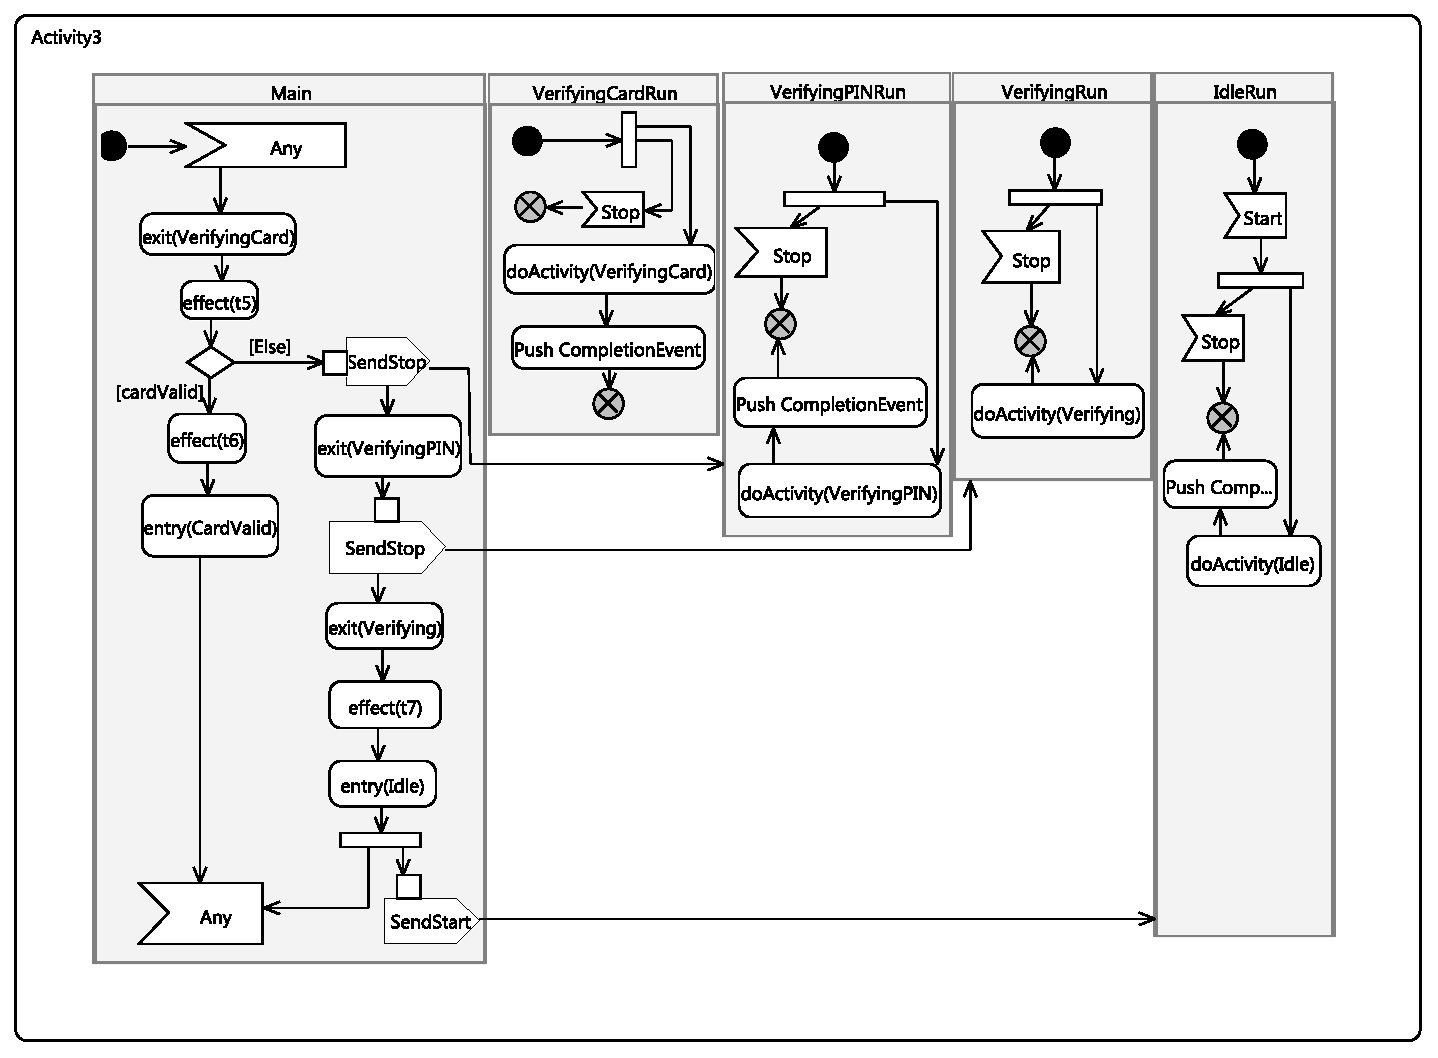
\includegraphics[clip, trim=1.5cm 1.6cm 1.6cm 1cm, width=1.03\columnwidth]{figures/ThreadingExample2.pdf}
	\caption{Concurrency of the ATM when \ti{doActivity} of \ti{VerifyingCard} completes before that of \ti{VerifyingPIN}}
	\label{fig:threading2}
\end{figure}

\paragraph{Thread-based design of generated code}
Each NDA is run in parallel with the main thread which reads and dispatch events from the event queue. 
Each is associated with a thread which is initialized at the state machine initialization moment. 
The number of threads associated with NDAs is therefore equal to that of the NDAs.
The design of threads is based on the thread pool pattern, which initializes all threads at once, and the paradigm "wait-execute-wait". 
In the latter, a thread \tb{waits} for a signal to \tb{execute} its associated method and goes back to the \tb{wait} point if it receives a stop signal or its associated method completes. 
An NDA is one of the followings:
\begin{itemize}
	\item \ti{doActivity} of each state if has. The number of \ti{doActivity} $n_{do} = \#\{s \in V|\exists doActivity(s)\}$
	
	\item Sleep function associated with a \ti{TimeEvent} which counts ticks and emits a \ti{TimeEvent} once completes: $n_{te} = \#\{e \in E|\ti{e is a time event}\}$.
	
	\item Change detect function associated with a \ti{ChangeEvent} which observes a variable or a boolean expression and pushes an event to the queue if changes happen: $n_{che} = \#\{e \in E|\ti{e is a change event}\}$.
\end{itemize} 

Therefore, the concurrency has the number of initial threads $n_{threads} = n_{do} + n_{te} + n_{che}$ plus a main thread which sends start and stop signals to these initial threads. 

Now we consider spontaneous threads which are created by \ti{FORK} to run DAs, joined until and destroyed once DAs complete. The followings describe different types of DAs:

\begin{itemize}
	\item Actions executed when entering/exiting an orthogonal region, which can be: execute a chain of transition effects contained by the region before entering a stable sub-state or exiting the region completely: $n_{region threads} = \#\{r \in \mathcal{R}|ctner(r).kind=concurrent\}$
	
	\item Effects of transitions outgoing from a $fork$ and those incomings to a $join$: \\
	$\mathcal{J} = \{v \in V|v.kind=join\}$ \\
	$\mathcal{F} = \{v \in V|v.kind=fork\}$ \\
	$$n_{FJ\_threads} = \sum_{v \in \mathcal{F}} {\#T_{outs}(v)} + \sum_{v \in \mathcal{J}} {\#T_{ins}(v)}$$.
\end{itemize}

The spontaneous threads follow a paradigm in which if a thread $parent$ creates a set of threads $children$, $parent$ must wait until $children$ complete their associate methods. These threads are created in one of the following cases:

\begin{itemize}
	\item Having multiple transitions outgoing from a \ti{fork}, for each transition effect, a thread is created by \ti{FORK}
	
	\item Entering a concurrent state $s$, after the execution of $entry(s)$, a thread is also created for each orthogonal region. 
	
	\item Exiting a concurrent state $s$, before the execution of $exit(s)$, a thread is also created for each region to exit the corresponding active sub-state. 
\end{itemize}

\paragraph{Example of generated code}

 


 



\section{\uppercase{Empirical Study}}
\label{sec:exp}
The pattern is implemented in Papyrus Designer \cite{PapyrusDesigner}, which is an extension of the UML modeling tool Papyrus \cite{cealistpapyrus}.
Papyrus Designer supports component-based modeling and code generation. 
The behavior of a component in Papyrus Designer is described by using UML State Machines.
The tool allows to use some time notions from the MARTE profile to specify time events.
C++ code is generated and runs within POSIX systems such as Ubuntu, in which Pthreads are used for implementing threads for concurrency. 
This section reports our experiments with Papyrus Designer on the semantic-conformance and efficiency of generated code.

\subsection{Semantic conformance of runtime execution}
\label{subsec:exp1}
This section presents our results found during experiments with our tool to answer the following research question.

\noindent
	\begin{mdframed}[backgroundcolor=blue!5]
		\small
		\tb{\ti{Research question 1:}} \ti{Is the runtime execution of code generated from USMs by our tool semantic-conformant to PSSM?}
	\end{mdframed}


To evaluate the semantic conformance of runtime execution of generated code, we use a set of examples provided by Moka \cite{moka}, which is a model execution engine offering PSSM (and also part of the Papyrus modeler). 
Fig. \ref{fig:semanticconformance} shows our method. 
%We first use our code generator to generate code (Step (1)) from the Moka example model set. 
%Step (2) simulates the examples by using Moka to extract the sequence (\tb{Traces 1}) of observed traces including executed actions. 
%The sequence (\tb{Traces 2}) is also obtained through the runtime execution of the code generated in Step (1). 
%The code is semantic-conformant if \tb{Traces 1} and \tb{Traces 2} are the same \cite{Blech2005}. %The current version of Moka does not support simulation for \ti{TimeEvent} and history pseudo states, we therefore leave experiments for \ti{TimeEvent} as future work.
The latter consists of the following steps:

\begin{description}
	\item[Step 1] For a \tb{State machine} from the Moka example set, we use our code generation tool to generate code.
	
	
	\item[Step 2] We simulate the execution of the \tb{State machine} by using Moka to extract a sequence \tb{Trace 1} of observed traces including executed actions.
	
	\item[Step 3] The sequence (\tb{Traces 2}) is obtained through the runtime execution of the code generated in Step 1.
	
	\item[Step 5] \ttt{Trace 1} and \ttt{Trace 2} are compared. The code is semantic-conformant if \tb{Traces 1} and \tb{Traces 2} are the same \cite{Blech2005}. 
\end{description}

%Within our scope as previously defined 30 examples of the Moka example set are tested. \ti{SimTraces} and \ti{RTTraces} for each case are the same. 
%This indicates that, within our study scope, the runtime execution of code generated by our generator can produce traces semantically equivalent to those obtained via simulation. 
The PSSM test suite consists of 66 test cases for different state macchine element types.
The results are promising: our tool passes 62/66 tests including: behavior (5/6), choice (3/3), deferred events (6/6), entering (5/5), exiting (4/5), entry(5/5), exit (3/3), event (9/9), final state (1/1), fork (2/2), join (2/2), transition (11/14), terminate (3/3), others (2/2).  
In fact, our tool fails with some tests containing transitions (1) from an \ttt{entry point} to an \ttt{exit point} or (2) from an entry point/exit point to itself. 
This is, as our observation, rarely used in practice because of the contradictory semantics of \ti{entry points} and \ti{exit points} as previously discussed. 
%Furthermore, as the UML specification says that transitions outgoing from an \ttt{entry point} of a composite state should end on one of the sub-vertexes.

The results of this evaluation are not enough to prove that our pattern and tooling support preserves the UML State Machine execution properties but are a good hint that runtime execution of generated code is semantically correct (for all but the case identified above).


This evaluation methodology has the limitation that it is dependent on PSSM.
Currently, for event support, PSSM only specifies signal events.
For pseudo-states, histories are not supported.
Thus, our evaluation result is limited to the current specification of PSSM.

\begin{figure}
	\centering
	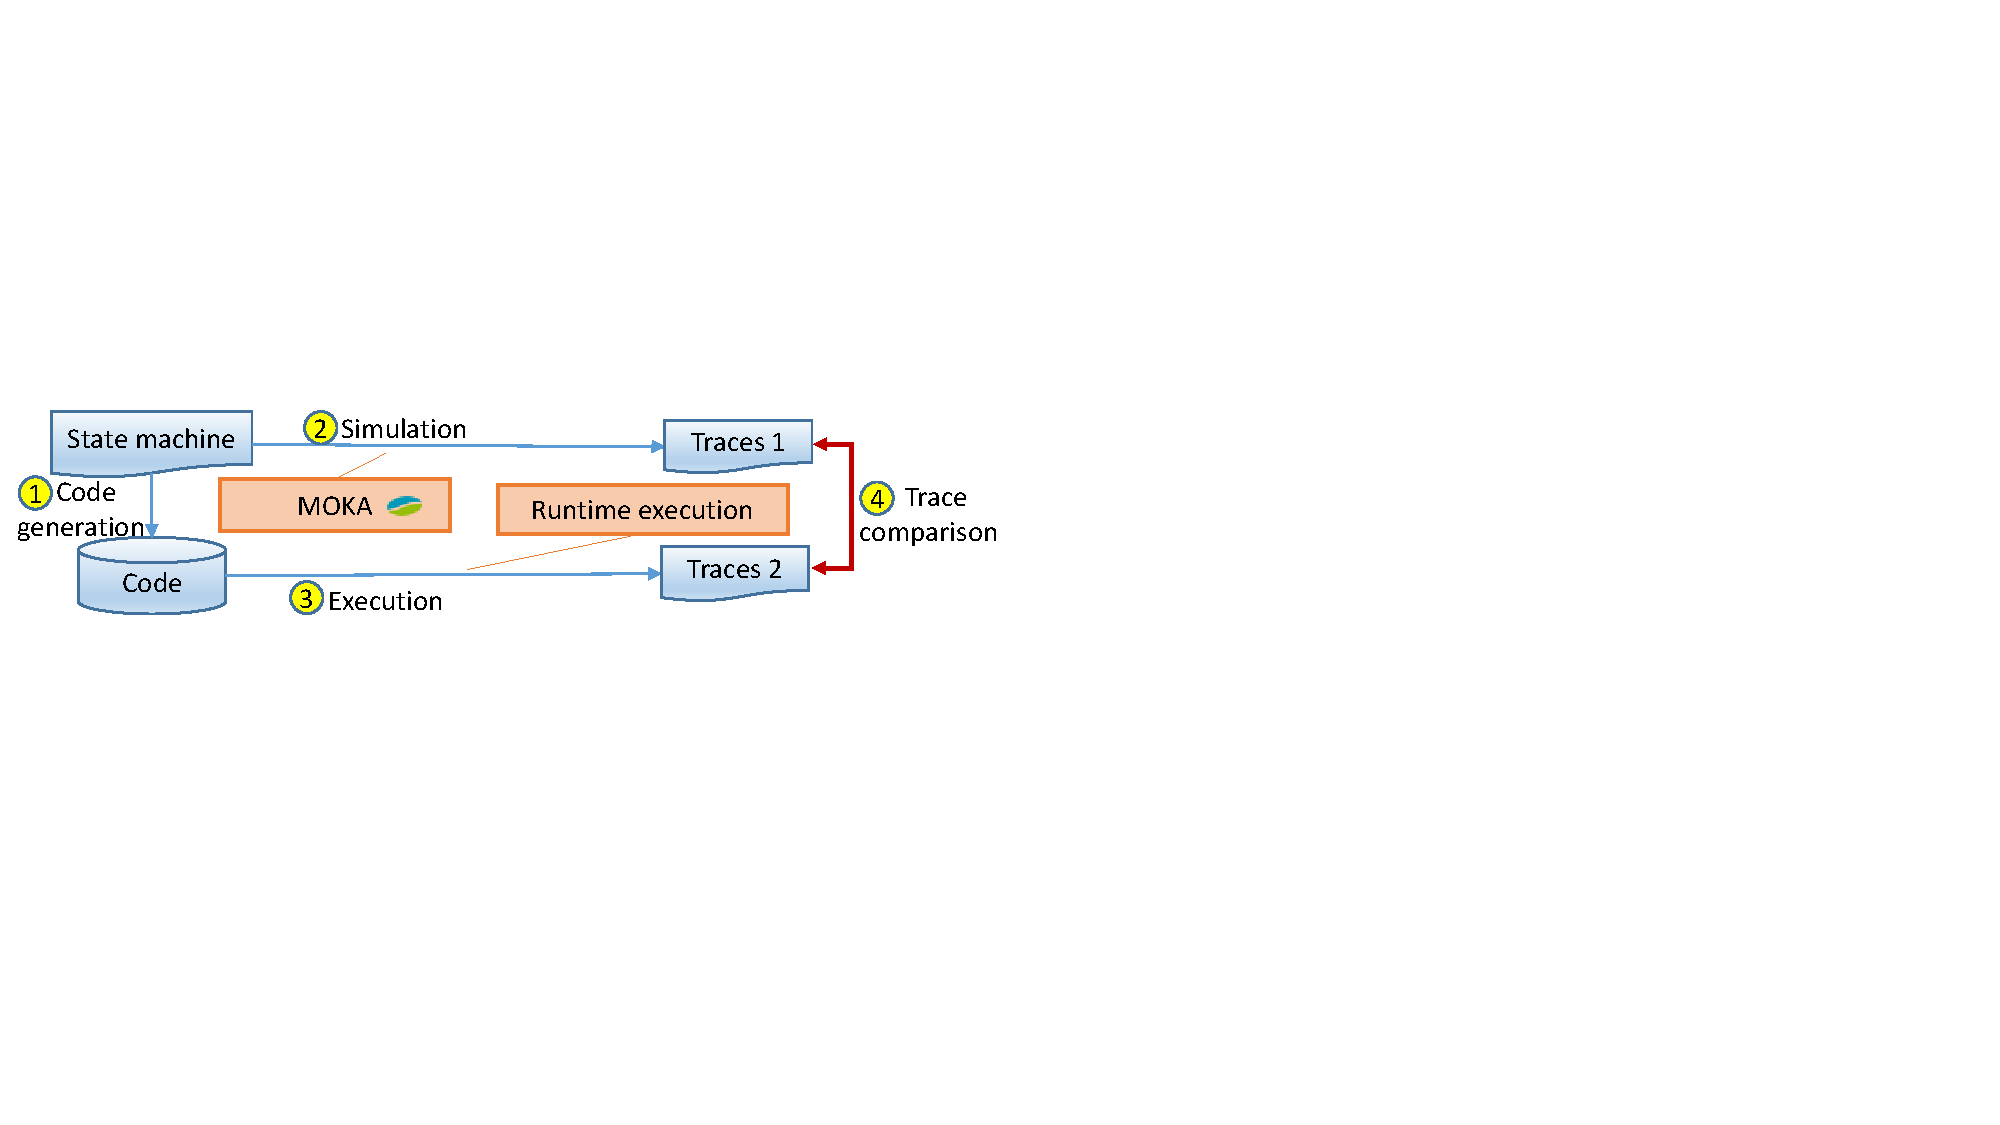
\includegraphics[clip, trim=0.2cm 8.6cm 16.7cm 6.9cm, width=\columnwidth]{figures/semanticconformance.pdf}
	\caption{Semantic conformance evaluation methodology} 
	\label{fig:semanticconformance}
\end{figure}		

\begin{comment}
\begin{table*}[]
	\centering
	\caption{Semantic-conformance test results (number of passed/total tests)}
	\label{table:semantic-test}
	\begin{tabular}{|l|l|l|l|l|l|l|l|l|l|l|l|l|l|}
		\hline
		Behavior & Choice & Deferred Events & Entering & Exiting & Entry & Exit & Event & Final & Fork & Join & Transition & Terminate & Others \\ \hline
		5/6&        3/3&         6/6        &    5/5      &    4/5     &  5/5     &   3/3   &    9/9    &   1/1    &   2/2   &   2/2   &      11/14      &    3/3       &    2/2    \\ \hline
	\end{tabular}
\end{table*}
\end{comment}

\vskip 0.1cm
\noindent
\tb{Threats to validity:}
%All test cases of the PSSM test suite are contained in a single model file.
%However, the input to our experiments requires a test case per model file.
Operation behaviors in PSSM are defined by activities while our prototype requires fine-grained behavior as blocks of code embedded into models.
Therefore, an internal threat is that we manually re-create these tests and convert activities into programming language code.

\subsection{Benchmarks}
\label{subsec:exp3}
In this section, we present the results obtained through the experiments on some efficiency aspects of generated code to answer the following question.

%\noindent
%\tb{\ti{Research question 2:}} \ti{Runtime performance and memory usage is undoubtedly critical in real-time and embedded systems. 
%Particularly, in event-driven systems, the performance is measured by event processing speed. 
%Is the performance of code generated by our tool comparable existing approaches and use less memory?}


\begin{mdframed}[backgroundcolor=blue!5]
\small
\tb{\ti{Research question 2:}} \ti{Runtime performance and memory usage are undoubtedly critical in real-time and embedded systems. 
Particularly, in event-driven systems, the performance is measured by event processing speed. 
Are the performance and memory usage of code generated by our tool comparable to existing approaches?}
\end{mdframed}
%Specifically, our research question related to memory consumption and runtime performance of generated code is stated as the following. 
%\noindent
%\tb{RQ3:} \ti{}
%\noindent
%\tb{Experimental dataset:} 
Two state machine examples are obtained by the preferred benchmark used by the Boost C++ libraries \cite{boost} in \cite{benchmark}. One simple example only consists of atomic states and the other both atomic and composite states. 

We compared our tool with tools such as Sinelabore (which generates efficient code for Magic Draw \cite{Magicdraw}, Enterprise Architect \cite{EA}), Quantum Modeling (QM) \cite{qm} (which generates code for event-driven active object frameworks \cite{Lavender1996})%, which generate code from state machines
, Boost Statechart \cite{Statechart}, Meta State Machine (MSM) \cite{MSM}, C++ 14 MSM-Lite \cite{benchmark}, and functional programming like-EUML\cite{EUML}. 
%The tools are Sinelabore, which efficiently generates code from UML State Machines created by various modeling tools such as Magic Draw \cite{Magicdraw}, Enterprise Architect \cite{EA}, and QM \cite{QM}. 
%C++ libraries are Boost Statechart \cite{Statechart}, Meta State Machine (MSM) \cite{MSM}, MSM-Lite \cite{MSMLite}, and EUML \cite{euml}.

We used a Ubuntu virtual machine 64 bit hosted by a Windows 7 machine. 
For each tool, we created two applications corresponding to the two examples, generated C++ code and compiled it in two modes: normal (N), by default GCC compiler; and optimal (O) with GCC optimization options -O2 -s. 
11 millions of events are generated and processed by the simple example and more than 4 millions for the composite example. 
%More than 4 millions of events are processed by the composite example. 
Processing time is measured for each case. 

\subsubsection{Performance} 
Fig. \ref{fig:boxplot} shows the event processing performance of the approaches for the two benchmarks.
%Table \ref{table-speed} shows the median of event processing time. 
In the normal compilation mode ( postfix N), Boost Statechart, MSM, MSMLite, EUML are quite slow and not displayed in the box-plot. 
%Only Sinelabore and QM are performantly comparable with our approach. 
  
%Boxplots in Fig. \ref{fig:boxplotsimple} and \ref{fig:boxplotcomposite} compare the performance of these approaches to that of our approach for the two examples, respectively. 
%In both of the simple and composite examples, 

%Our approach processes faster around 40 milliseconds than the fastest approach within the scope of the experiment.
%Even without GCC optimizations, code generated by our approach significantly runs faster than that of EUML and QM with the optimizations. 
%When compiled with the optimizations, our approach improves the event processing speed. 
In both of the simple and composite benchmarks, in optimization mode (postfix O) MSMLite and our tool run faster than the others in the scope of the experiment.
The figure also shows that the optimization of GCC is significant.
In normal mode only the performance of Sinelabore, QM, and our tool is acceptable. 
The event processing speed of MSM, MSM\_Lite and EUML is too slow without GCC optimizations. 
%Even, in case of composite, our approach does not produce any slowness compared to the simple example. 


% Please add the following required packages to your document preamble:
% \usepackage{multirow}
\begin{comment}
\begin{table*}[]
	\centering
	\caption{Event processing speed in ms}
\label{my-label}
\begin{tabular}{|l|l|l|l|l|l|l|l|l|l|l|l|l|l|l|l|l|}
	\hline
	\multicolumn{1}{|c|}{\multirow{2}{*}{Test}} & \multicolumn{2}{c|}{SC} & \multicolumn{2}{c|}{MSM} & \multicolumn{2}{c|}{MSM-Lite} & \multicolumn{2}{c|}{EUML} & \multicolumn{2}{c|}{Sinelabore} & \multicolumn{2}{c|}{QM} & \multicolumn{2}{l|}{Umple} & \multicolumn{2}{c|}{Our approach} \\ \cline{2-17} 
	\multicolumn{1}{|c|}{}                      & N           & O         & N            & O         & N              & O            & N            & O          & N               & O             & N          & O          & N            & O           & N                & O              \\ \hline
	Simple                                      & 13705,75    & 1658,1    & 5249,57      & 70,63     & 833,67         & 79,37        & 10867,93     & 109,97     & 141,03          & 79,93         & 285,9      & 229,27     & X            & X           & 106,87           & 25,37          \\ \hline
	Composite                                   & 5353,03     & 820,63    & 3546,1       & 46,73     & 516,87         & 65,17        & 4225,57      & 92,3       & 100,03          & 86,03         & 146,23     & 97,57      & X            & X           & 36,47            & 1,40           \\ \hline
\end{tabular}
\end{table*}
\end{comment}

\begin{comment}
\begin{table*}[]
	\centering
	\caption{Event processing speed in ms}
	\label{table-speed}
	\begin{tabular}{|l|l|l|l|l|l|l|l|l|l|l|l|l|l|l|l|l|}
		\hline
		\multicolumn{1}{|c|}{\multirow{2}{*}{Test}} & \multicolumn{2}{c|}{SC} & \multicolumn{2}{c|}{MSM} & \multicolumn{2}{c|}{MSM-Lite} & \multicolumn{2}{c|}{EUML} & \multicolumn{2}{c|}{Sinelabore} & \multicolumn{2}{c|}{QM} & \multicolumn{2}{l|}{Umple} & \multicolumn{2}{c|}{Our approach} \\ \cline{2-17} 
		\multicolumn{1}{|c|}{}                      & N           & O         & N            & O         & N              & O            & N            & O          & N               & O             & N          & O          & N            & O           & N                & O              \\ \hline
		Simple                                      & 13706    & 1658    & 5250      & 71     & 834         & 79        & 10868     & 110     & 141          & 80         & 286      & 229     & X            & X           & 107           & 25,4          \\ \hline
		Composite                                   & 5353     & 821    & 3546       & 47     & 517         & 65        & 4225,6      & 92       & 100          & 86         & 146     & 98      & X            & X           & 36,5            & 1,40           \\ \hline
	\end{tabular}
\end{table*}
\end{comment}


\begin{comment}
\begin{table*}[]
	\centering
	\caption{Event processing speed in ms}
	\label{table-speed}
	\begin{tabular}{|l|l|l|l|l|l|l|l|l|l|l|l|l|l|l|}
		\hline
		\multicolumn{1}{|c|}{\multirow{2}{*}{Test}} & \multicolumn{2}{c|}{SC} & \multicolumn{2}{c|}{MSM} & \multicolumn{2}{c|}{MSM-Lite} & \multicolumn{2}{c|}{EUML} & \multicolumn{2}{c|}{Sinelabore} & \multicolumn{2}{c|}{QM} & \multicolumn{2}{c|}{PSM} \\ \cline{2-15} 
		\multicolumn{1}{|c|}{}                      & N           & O         & N            & O         & N              & O            & N             & O         & N               & O             & N          & O          & N           & O          \\ \hline
		Simple                                      & 13706       & 1658      & 5250         & 71        & 834            & 79           & 10868         & 110       & 141             & 80            & 286        & 229        & 107         & 25,4       \\ \hline
		Composite                                   & 5353        & 821       & 3546         & 47        & 517            & 65           & 4225,6        & 92        & 100             & 86            & 146        & 98         & 36,5        & 1,40       \\ \hline
	\end{tabular}
\end{table*}
\end{coment}


\begin{comment}
\begin{figure}
	\centering
	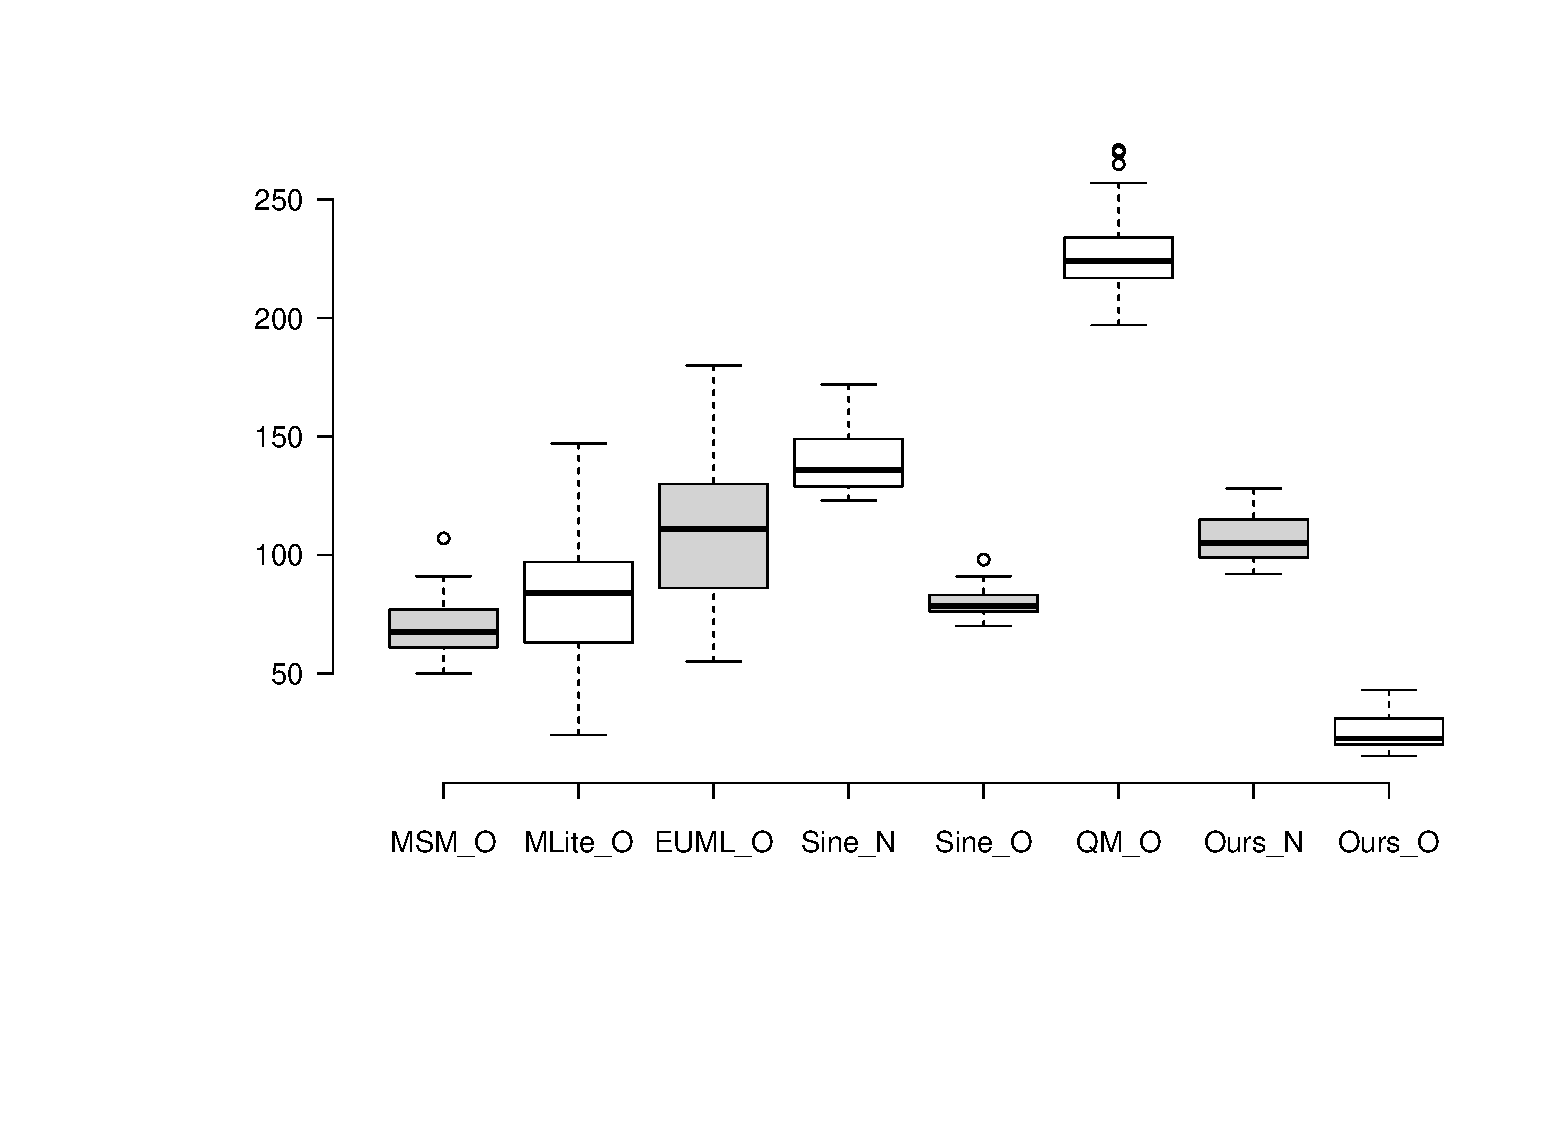
\includegraphics[clip, trim=4.2cm 4.6cm 1.7cm 2.3cm, width=\columnwidth]{figures/boxplotsimple.pdf}
	\caption{Event processing speed for the \ti{Simple} benchmark} 
	\label{fig:boxplotsimple}
\end{figure}

\begin{figure}
	\centering
	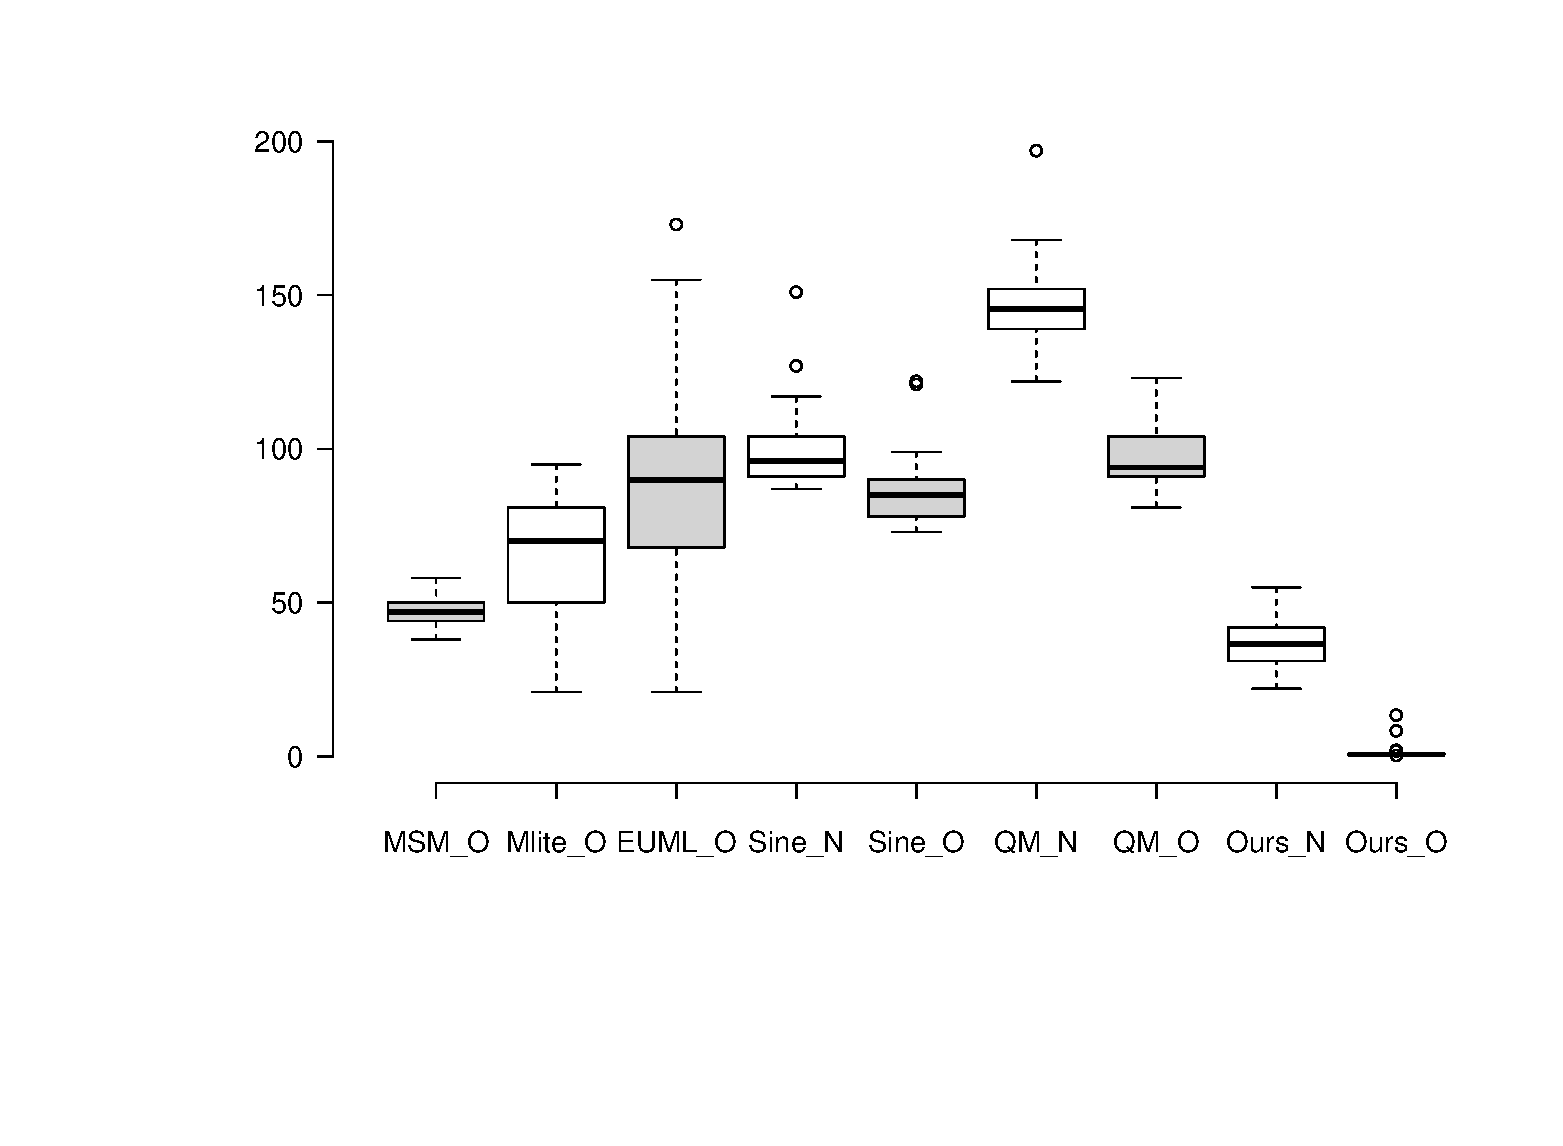
\includegraphics[clip, trim=4.2cm 4.6cm 1.7cm 1.8cm, width=\columnwidth]{figures/boxplotcomposite.pdf}
	\caption{Event processing speed for the \ti{Composite} benchmark} 
	\label{fig:boxplotcomposite}
\end{figure}
\end{comment}

\begin{figure}
	\centering
	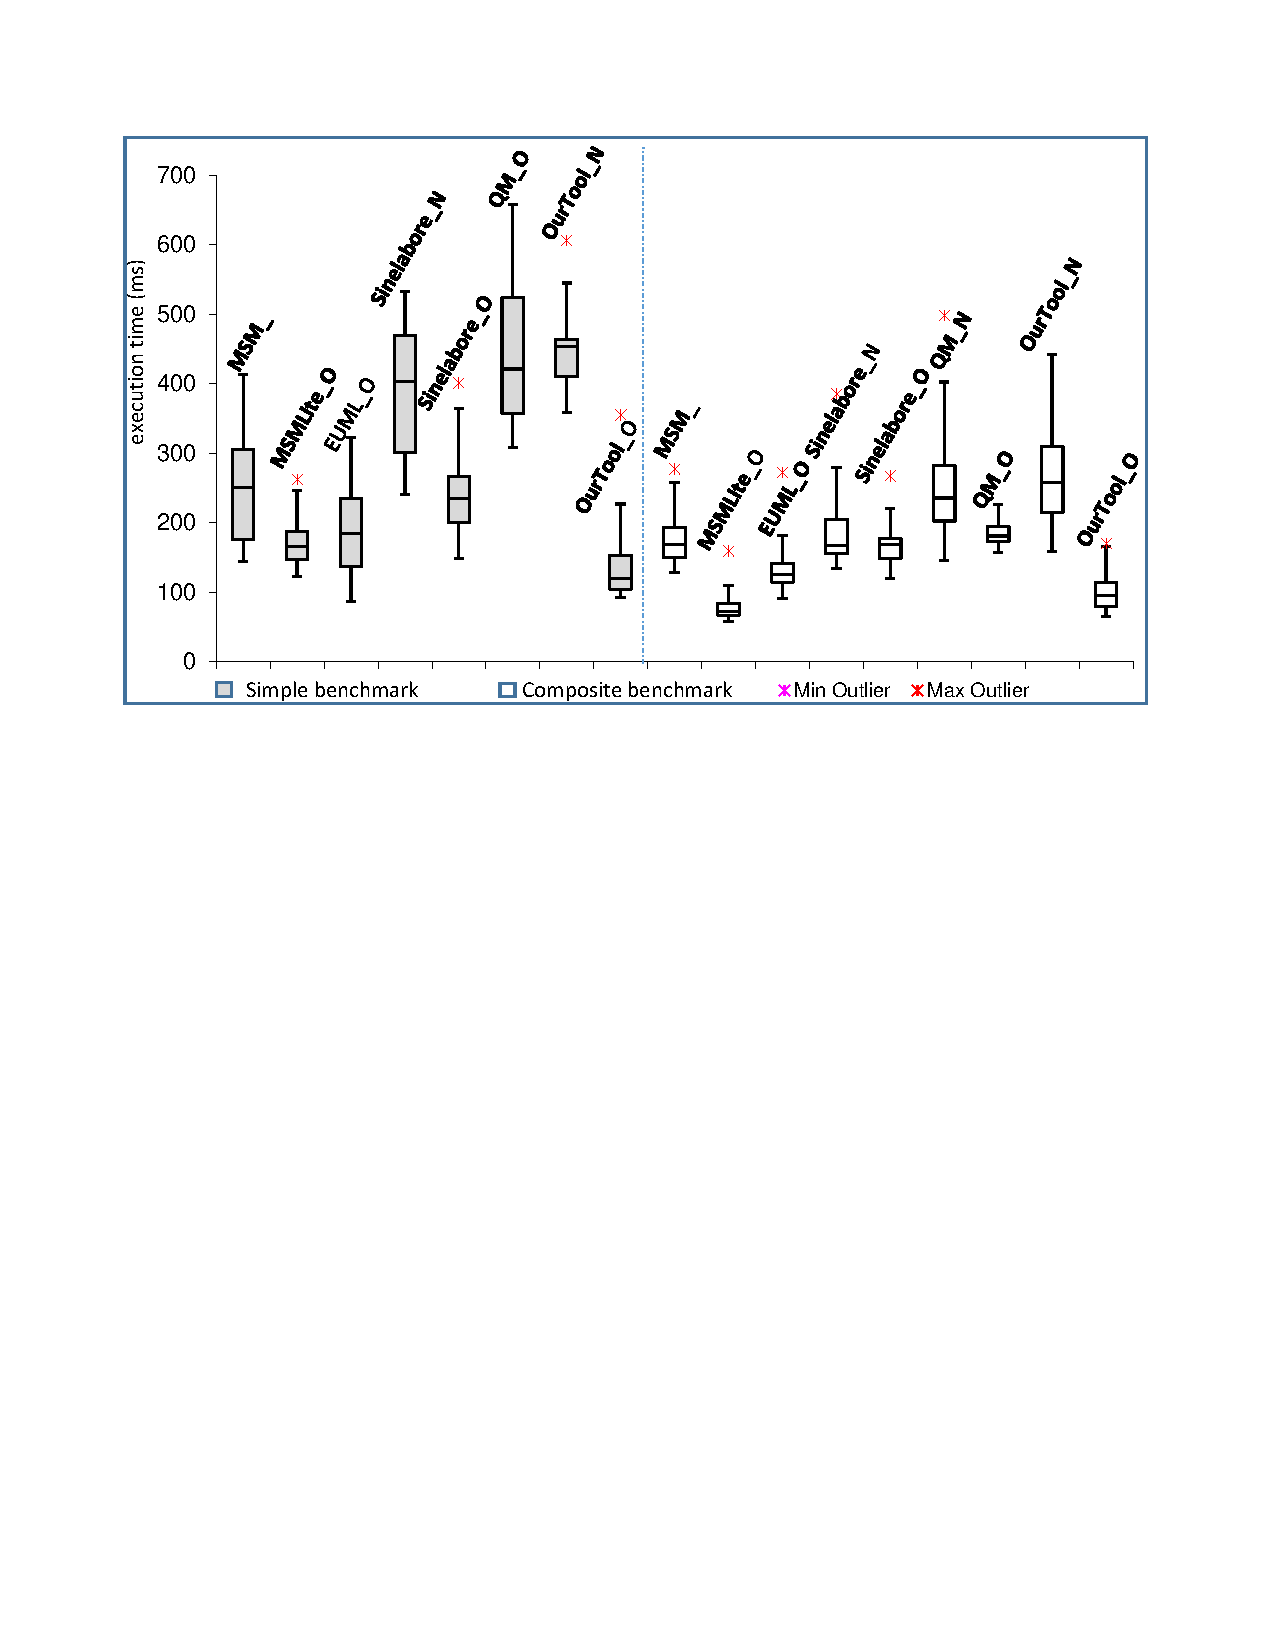
\includegraphics[clip, trim=2.1cm 16.0cm 1.7cm 2.3cm, width=\columnwidth]{experiments/box-plot-mine.pdf}
	\caption{Event processing speed for the benchmarks} 
	\label{fig:boxplot}
\end{figure}

\subsubsection{Memory usage} 
Table \ref{table-size} shows the executable size for the examples compiled in two modes.
Without optimization, Sinelabore generates the smallest executable size while our approach takes the second place.
In GCC optimization mode, MSMLite, Sinelabore and our approach require less static memory than the others. 

Let's look closer at the event processing performance in optimization mode in terms of time medians.
Fig. \ref{fig:comparepercentage} shows the figures of the two benchmarks, relative to the performance of Sinelabore (normalized to 100\%).
For the simple (blue) benchmark, our approach (51.3\%) is the fastest. 
For the composite (red) benchmark, with the support of C++14, the performance in MSMLite (42.7\%) is the fastest and ours is the second.   

For runtime memory consumption, we use the Valgrind Massif profiler \cite{Massif,nethercote2007valgrind} to measure memory usage. 
Table \ref{table:usage} shows the memory consumption measurements including stack and heap usage for the composite example. 
Compared to others, code generated by our approach requires a slight overhead with regard to runtime memory usage (0.35KB).
This is predictable since the major part of the overhead is used for C++ multi-threading using POSIX Threads and resource control using POSIX Mutex and Condition. 
However, the overhead is small and acceptable (0.35KB). 


\begin{comment}
\begin{table*}[]
	\centering
	\caption{Executable size in Kb}
	\label{table-size}
	\begin{tabular}{|l|l|l|l|l|l|l|l|l|l|l|l|l|l|l|l|l|}
		\hline
		\multirow{2}{*}{Test} & \multicolumn{2}{c|}{SC} & \multicolumn{2}{c|}{MSM} & \multicolumn{2}{c|}{MSM-Lite} & \multicolumn{2}{c|}{EUML} & \multicolumn{2}{c|}{Sinelabore} & \multicolumn{2}{c|}{QM} & \multicolumn{2}{l|}{Umple} & \multicolumn{2}{c|}{Our approach} \\ \cline{2-17} 
		& N           & O         & N           & O          & N              & O            & N            & O          & N              & O              & N          & O          & N            & O           & N               & O               \\ \hline
		Simple                & 320      & 63,9     & 414,6      & 22,9      & 107,3         & 10,6        & 2339      & 67,9      & 16,5          & 10,6          & 22,6      & 10,5      &       X       &       X      & 21,5           & 10,6           \\ \hline
		Composite             & 435,8      & 84,4     & 837,4      & 31,1      & 159,2         & 10,9        & 4304,8      & 92,5      & 16,6          & 10,6          & 23,4      & 21,5      & X           & X          & 21,6           & 10,6           \\ \hline
	\end{tabular}
\end{table*}
\end{comment}


%ToDo: test speed with dispatch function
% Please add the following required packages to your document preamble:
% \usepackage{multirow}
\begin{table*}[]
	\scriptsize
	\centering
	\caption{Executable size in KB}
	\label{table-size}
	\begin{tabular}{|l|l|l|l|l|l|l|l|l|l|l|l|l|}
		\hline
		\multirow{2}{*}{Test} & \multicolumn{2}{c|}{MSM} & \multicolumn{2}{c|}{MSM-Lite} & \multicolumn{2}{c|}{EUML} & \multicolumn{2}{c|}{Sinelabore} & \multicolumn{2}{c|}{QM} & \multicolumn{2}{c|}{Our tool} \\ \cline{2-13} 
		& N           & O          & N              & O            & N            & O          & N              & O              & N          & O          & N            & O           \\ \hline
		Simple                & 414,6       & 22,9       & 107,3          & 10,6         & 2339         & 67,9       & 16,5           & 10,6           & 22,6       & 16,6       & 21,5         & 10,6        \\ \hline
		Composite             & 837,4       & 31,1       & 159,2          & 10,9         & 4304,8       & 92,5       & 16,6           & 10,6           & 23,4       & 21,5       & 21,6         & 10,6        \\ \hline
	\end{tabular}
\end{table*}

%\subsubsection{Runtime memory consumption}
\begin{comment}
\begin{table}[]
	\centering
	\caption{Runtime memory consumption in KB. Columns (1) to (7) are SC, MSM, MSM-Lite, EUML, Sinelabore, QM, and our approach, respectively.}
	\label{table:usage}
	\begin{tabular}{|l|l|l|l|l|l|l|l|l|}
		\hline
		Test      & (1)    & (2)  & (3) & (4) & \begin{tabular}[c]{@{}l@{}}(5)\end{tabular} & (6)    & \begin{tabular}[c]{@{}l@{}}(7)\end{tabular} \\ \hline
		Composite & 76.03 & 75.5 & 75.8  & 75.5 & 75.8                                                  & 75.7      & 76.38                                                   \\ \hline
	\end{tabular}
\end{table}
\end{comment}

\begin{table}[]
	\scriptsize
	\centering
	\caption{Runtime memory consumption in KB. Columns from left to right are SC, MSM, MSM-Lite, EUML, Sinelabore, QM, and Our tool, respectively.}
	\label{table:usage}
	\begin{tabular}{|l|l|l|l|l|l|l|}
		\hline
		76.03 & 75.5 & 75.8 & 75.5 & 75.8 & 75.7 & 76.38 \\ \hline
	\end{tabular}
\end{table}


\begin{figure}
	\centering
	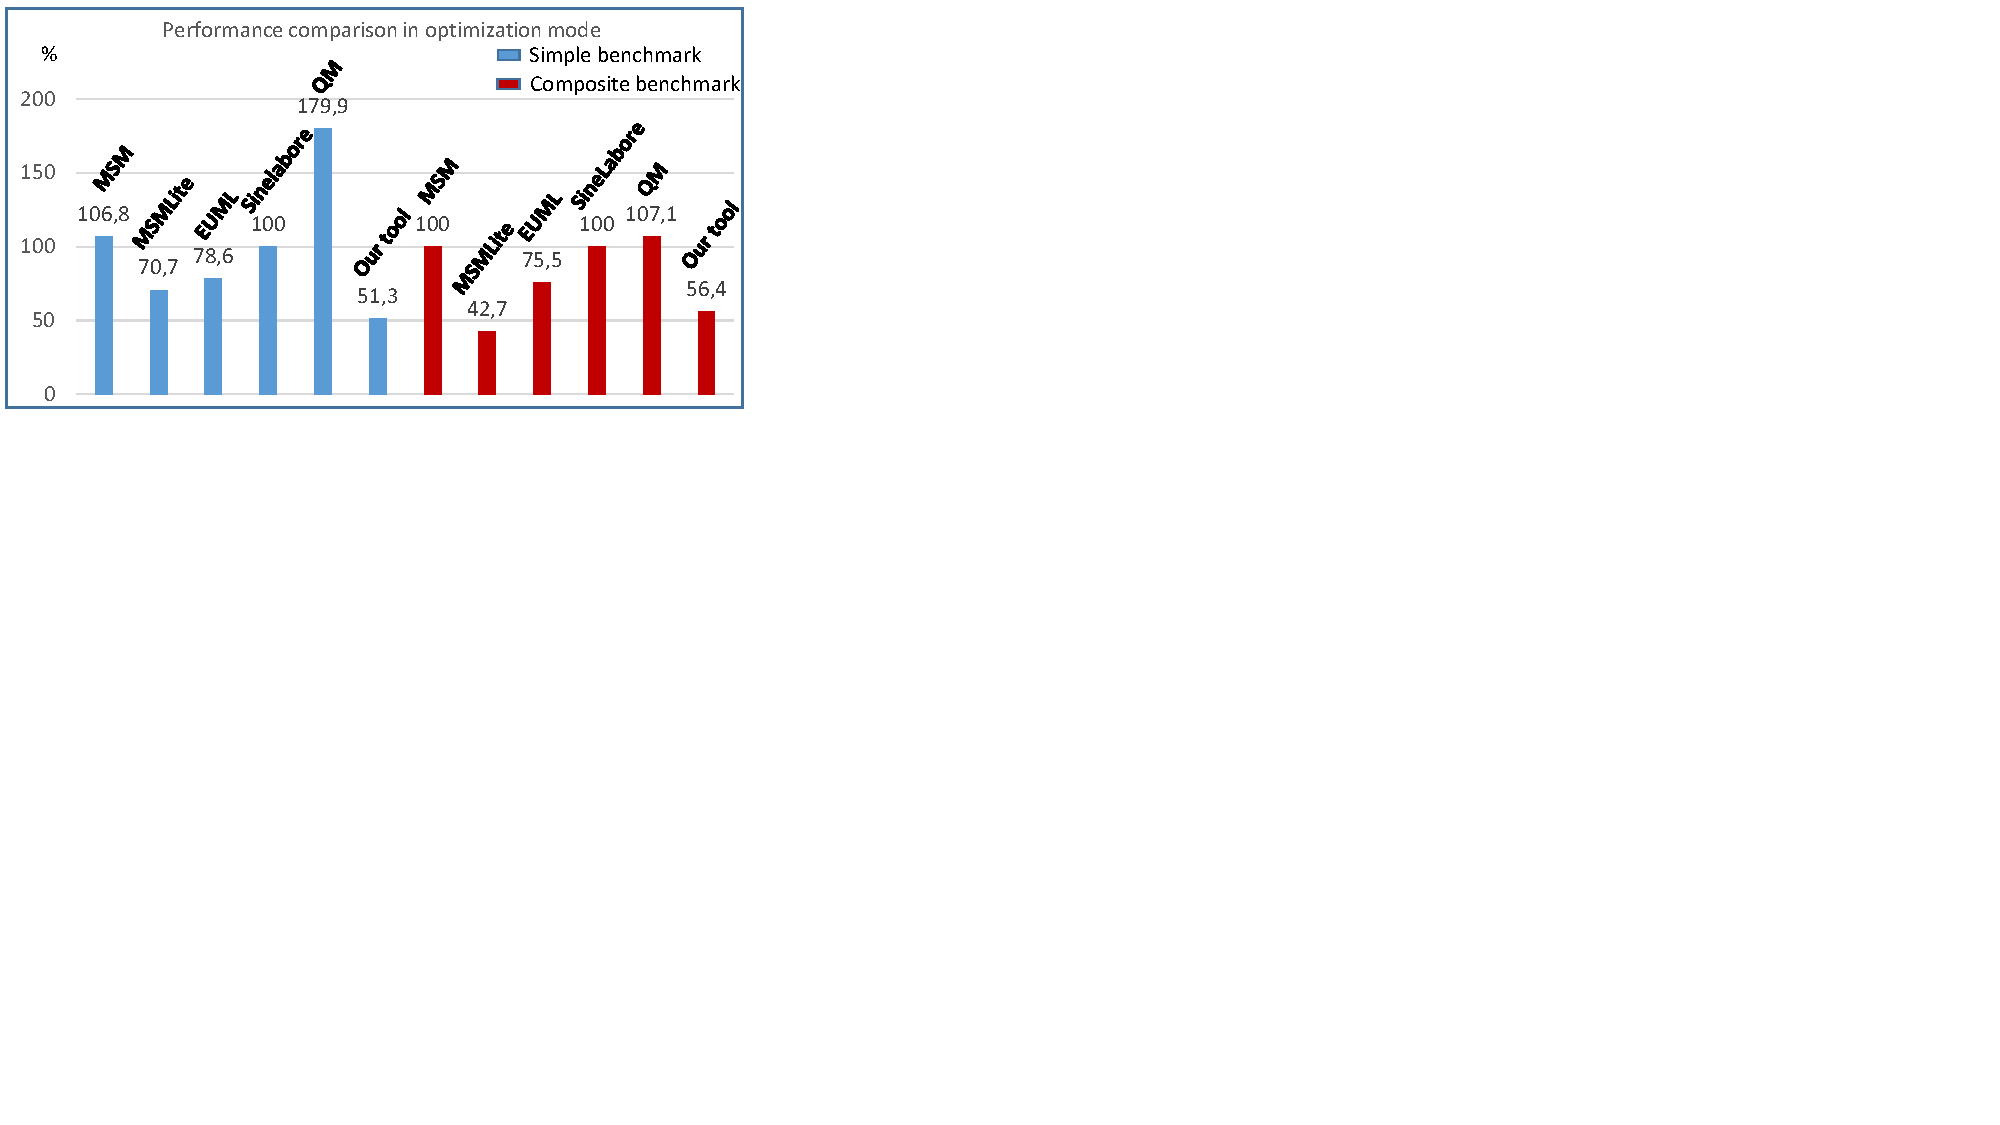
\includegraphics[clip, trim=0cm 12.1cm 21.0cm 0cm, width=\columnwidth]{experiments/comparepercentage.pdf}
	\caption{Event processing performance in optimization mode} 
	\label{fig:comparepercentage}
\end{figure}


%\lipsum[1-6]


%\lipsum[1-6]

\section{\uppercase{Related work}}
\label{sec:relatedwork}
Code generation from state machines has received a lot of attention in automated software development. 
This section mentions some existing code generation patterns and how our approach differs. 
A systematic review of several proposals is presented in \cite{Domnguez2012}. 
%Main approaches including switch/if, state table and state pattern are investigated.

%Switch/if is the most intuitive technique implementing a "flat" state machine. Two types of switch/if are supported. The first one uses a scalar variable representing the current active state \cite{Booch1998}. A method for each event processes the variable as a discriminator in switch/if statement. The second one uses a double nested switch/if and has two variables to represent the current active state and the event to be processed \cite{Douglass1999}. The latter are used as the discriminators of an outer switch statement to select between states and an inner one/if statement to decide how the event should be processed. The behavior code of the two types is put in one file or class. This practice makes code cumbersome, complex, difficult to read and less explicit when the number of states grows or the state machine is hierarchical. Furthermore, the first approach lets the code scatter in different places. Therefore, maintaining or modifying such code of complex systems is very difficult.

Switch/if is the most intuitive technique for implementing a "flat" state machine. 
It either uses a scalar variable \cite{Booch1998} and a method for each event, or using two variables as the active state and the incoming event used as the discriminators of an outer switch statement to select between states and an inner one/if statement, respectively. 
The state table approach \cite{Douglass1999} uses one dimension for representing states and the other one for all possible events. 
These approaches require a transformation from hierarchical to flatten state machines. 
However, these approaches are hardly applied to state machines containing pseudo states such as deep history or join/fork.  
%Each cell of the table is associated with a function pointer meaning that the state associated with a dimension index of the cell is triggered by the event associated with the other dimension. 
%The behavior code of these techniques is put in one file or class. This practice makes code cumbersome, complex, difficult to read and less explicit when the number of states grows or the state machine is hierarchical. 
%Therefore, maintaining or modifying such code of complex systems is very difficult. 
%Furthermore, these approaches requires every transition must be triggered by at least an event. This is obviously only applied to a small sub-set of USMs.  

The object-oriented state pattern \cite{Shalyto2006,Douglass1999} transforms a state into a class and an event into a method. 
Events are processed by delegating from the class containing the state machine to its sub-state classes. 
Separation of states in classes makes the code more readable and maintainable. Unfortunately, this technique only supports flat state machines. 
This pattern is extended in \cite{niaz_mapping_2004} to support hierarchical state machines. 
Recently, a double-dispatch (DD) pattern presented in \cite{spinke_object-oriented_2013} extends \cite{niaz_mapping_2004} to support maintainability by %as a new technique to implement state machines. 
representing states and events as classes, and transitions as methods. 
However, as the results shown in \cite{spinke_object-oriented_2013}, these patterns require much memory because of an explosion of the number of classes and use dynamic memory allocation, which is not preferred in embedded systems.
%However, the maintenance of the code generated by this approach is not trivial since it requires many small changes in different places. %This is impractical when dealing with large state machines. %Furthermore, similar to the state table, this approach also poses the requirement of having at least one event for transition.
It is worth noting that none of these approaches provides implementation for all of state machine pseudo states as well as events.

Tools such as \cite{sparxsystems_enterprise_2014,ibm_rhapsody} apply different patterns to generate code. 
However, as mentioned in Section \ref{sec:intro}, true concurrency, some pseudo-states, and UML events are not supported. 
FXU \cite{Pilitowski2007} is the most complete tool but generated code is heavily dependent on their own library and C\# is generated.

Umple \cite{Badreddin2014} is a textual UML programming language, which supports code generation for different languages such as C++ and Java from state machines.
However, Umple does not support pseudo states such as fork, join, junction, and deep history, and local transitions.
Furthermore, only call events and time events are specified in Umple.

Our approach combines the classical switch/if pattern, to produce small footprint, and the pattern in \cite{niaz_mapping_2004}, to preserve state hierarchy.
Furthermore, we define pattern to transform all of USM concepts including states, pseudo states, transitions, and events.
Therefore, users are flexible to create there USM conforming to UML without restrictions.

%Our generation approach relies on and extends this approach. The latter profits the polymorphism of object-oriented languages. %provides some 1-1 mappings from state machines to object-oriented code and the implementation technique 
%is not dependent on a specific programming language. 
%However, DD does not deal with triggerless transitions and different event types supported by UML such as \ti{CallEvent}, \ti{TimeEvent} and \ti{SignalEvent}. Furthermore, DD is not a code generation approach but an approach to manually implementing state machines.

\section{Conclusion}
\label{sec:conclusion}
%\lipsum[1]
%\input{sections/ack}
\bibliographystyle{abbrv}
\bibliography{refs}

\end{document}